% LaTeX source for ``การเรียนรู้ของเครื่องสำหรับเคมีควอนตัม (Machine Learning for Quantum Chemistry)''
% Copyright (c) 2022 รังสิมันต์ เกษแก้ว (Rangsiman Ketkaew).

% License: Creative Commons Attribution-NonCommercial-NoDerivatives 4.0 International (CC BY-NC-ND 4.0)
% https://creativecommons.org/licenses/by-nc-nd/4.0/

\chapter{วิธีคำนวณทางโครงสร้างเชิงอิเล็กทรอนิกส์}
\label{ch:el_strct}

\begin{figure}[H]
    \centering
    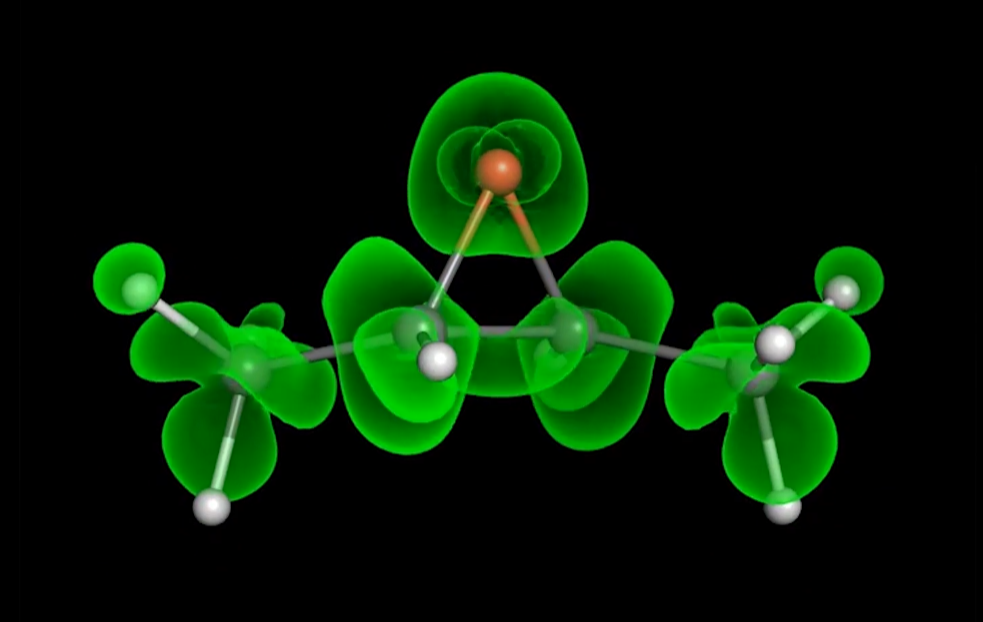
\includegraphics[width=0.75\linewidth]{fig/electron_density.png}
    \caption{ความหนาแน่นของอิเล็กตรอนของโมเลกุล 2,3-(S,S)-dimethyloxirane ซึ่งคำนวณด้วยวิธี Real-Time Density Functional Theory}
    \label{fig:elec_density}
\end{figure}

ส่วนที่สองของหนังสือเล่มนี้จะเกี่ยวข้องกับเคมีควอนตัมเป็นหลัก เคมีควอนตัมเป็นพื้นฐานสำคัญของการพัฒนาเทคนิคสำหรับการวิเคราะห์คุณสมบัติของโมเลกุลโดยนักเคมีนั้นส่วนใหญ่แล้วจะใช้เทคนิคทางสเปกโทรสโกปี เช่น Infrared (IR) Spectroscopy, Nuclear Magnetic Resonance (NMR) Spectroscopy, และ Scanning Probe Microscopy ซึ่งเทคนิคเหล่านี้ล้วนเกี่ยวข้องกับการคำนวณหาพลังงานในระดับโมเลกุล นอกจากนี้แล้วเคมีควอนตัมยังเกี่ยวข้องกับการศึกษาสถานะพื้น (Ground State) และสถานะกระตุ้น (Excited State) ของอะตอมแต่ละตัว รวมไปถึงการศึกษากลไกการเกิดปฏิกิริยาเคมีและสถานะทรานซิชั่น (Transition State) ที่เป็นสถานะที่เกิดขึ้นในการเปลี่ยนแปลงโครงสร้างของโมเลกุล การที่เราเข้าใจองค์ความรู้ขั้นพื้นฐานในระดับอะตอมและโมเลกุลนั้นทำให้เราประยุกต์ใช้และนำไปสู่การศึกษาคุณสมบัติของโมเลกุลในระดับที่ใหญ่ขึ้นได้ เช่น เทอร์โมไดนามิกส์ (Thermodynamics) และจลนศาสตร์เชิงเคมี (Chemical Kinetics) ซึ่งนำไปสู่การพัฒนาแบบจำลองทางคณิตศาสตร์ต่าง ๆ ซึ่งสามารถใช้คอมพิวเตอร์ในการศึกษาระบบที่เราสนใจได้ก่อนที่จะไปศึกษาจริงในห้องทดลอง

บทนี้ซึ่งเป็นบทแรกของส่วนที่สองนั้นผู้อ่านจะได้ศึกษาโครงสร้างเชิงอิเล็กทรอนิกส์ (Electronic Structure) ของโมเลกุล ซึ่งเป็นการศึกษาว่าอิเล็กตรอนที่อยู่ภายในอะตอมและโมเลกุลนั้นมีพฤติกรรมอย่างไรทั้งในสถาวะพื้นและสถาวะกระตุ้น โดยเราจะมาดูรายละเอียดของทฤษฎีควอนตัมในมุมมองของนักเคมีทฤษฎีรวมไปถึงการพัฒนาระเบียบวิธีการคำนวณเพื่อใช้ในการอธิบายอันตรกิริยาระหว่างอิเล็กตรอนและศึกษาคุณสมบัติของอะตอมและโมเลกุลต่อไป
\idxboth{โครงสร้างเชิงอิเล็กทรอนิกส์}{Electronic Structure}

%--------------------------
\section{ฟังก์ชันคลื่น}
\label{sec:wavefunction}
\idxboth{ฟังก์ชันคลื่น}{Wavefunction}
%--------------------------

%--------------------------
\subsection{ประวัติศาสตร์และความสำคัญของสมการชโรดิงเงอร์}
\label{ssec:schrodinger_eq}
\idxboth{ฟังก์ชันคลื่น!สมการชโรดิงเงอร์}{Wavefunction!Schr\"{o}dinger Equation}
%--------------------------

โมเลกุลเป็นหน่วยพื้นฐานของสิ่งต่าง ๆ รอบตัวเรา โมเลกุลก็คือกลุ่มของอะตอมหลาย ๆ อะตอมมารวมกันและในอะตอมนั้นเราสนใจพฤติกรรมของอิเล็กตรอนเป็นพิเศษ ในวิชากลศาสตร์ควอนตัมนั้นเราจะอธิบายพฤติกรรมของโมเลกุลโดยมุ่งเน้นไปที่อิเล็กตรอนซึ่งสามารถที่จะถูกอธิบายได้ด้วยฟังก์ชันทางคณิตศาสตร์ที่เรียกว่า \enquote{\textit{ฟังก์ชันคลื่น (Wavefunction)}} ซึ่งถูกพัฒนาขึ้นมาเพื่อเป็นแนวคิดสำหรับการอธิบายอิเล็กตรอนและระบบที่ประกอบไปด้วยอิเล็กตรอนหลายตัว โดยหนึ่งในสมการที่โด่งดังที่สุดสมการหนึ่งของวงการวิทยาศาสตร์นั่นคือสมการชโรดิงเงอร์ (Schr\"{o}dinger Equation)\autocite{schleich2013} ซึ่งนำเสนอโดยศาสตราจารย์ Erwin R. J. A. Schr\"{o}dinger (นักฟิสิกส์เชื้อสายออสเตรีย-ไอริช ซึ่งในขณะนั้นดำรงตำแหน่งอยู่ที่ University of Zurich) สำหรับการอธิบาย Wavefunction โดย Schr\"{o}dinger ได้ตีพิมพ์บทความงานวิจัยในวารสาร Annalen der Physik\footnote{ปัจจุบันนี้วารสาร Annalen der Physik ยังตีพิมพ์บทความวิชาการอย่างต่อเนื่อง} ในปี ค.ศ. 1926 ที่ต่อเนื่องกันเป็นจำนวน 4 บทความในซีรีย์ที่ชื่อว่า \textit{Quantisierung als Eigenwertproblem} โดยบทความฉบับแรกนั้นเป็นการนำเสนอสมการ \textbf{Time-independent Schr\"{o}dinger Equation}\autocite{schrodinger1926} และในเวลาต่อมา Schr\"{o}dinger ก็สามารถพิสูจน์หารูปแบบของสมการ \textbf{Time-dependent Schr\"{o}dinger Equation} และตีพิมพ์ในบทความฉบับที่ 4 ได้สำเร็จ\autocite{schrodinger1926a} โดยสมการชโรดิงเงอร์ถูกนำมาใช้ในการศึกษาระบบทางกลศาสตร์ควอนตัมซึ่งการแก้สมการชโรดิงเงอร์ได้นั้นจะทำให้ได้มาซึ่งผลเฉลยของสมการคณิตศาสตร์ที่อธิบาย Wavefunction ได้นั่นเอง

จากผลงานดังกล่าวทำให้ศาสตราจารย์ Erwin Schr\"{o}dinger ได้รับรางวัลโนเบลสาขาฟิสิกส์ ค.ศ. 1933 ร่วมกับศาสตราจารย์ Paul A. M. Dirac (ศาสตราจารย์ที่ University of Cambridge) ซึ่งเป็นหนึ่งในผู้บุกเบิกกลศาสตร์ควอนตัมและการพัฒนาสมการดิแรก (Dirac Equation) ซึ่งถูกนำมาใช้อธิบายพฤติกรรมของแฟร์มิออน (Fermions)\footnote{อ้างอิง \url{https://www.nobelprize.org/prizes/physics/1933/summary}}

\begin{figure}[H]
    \centering
    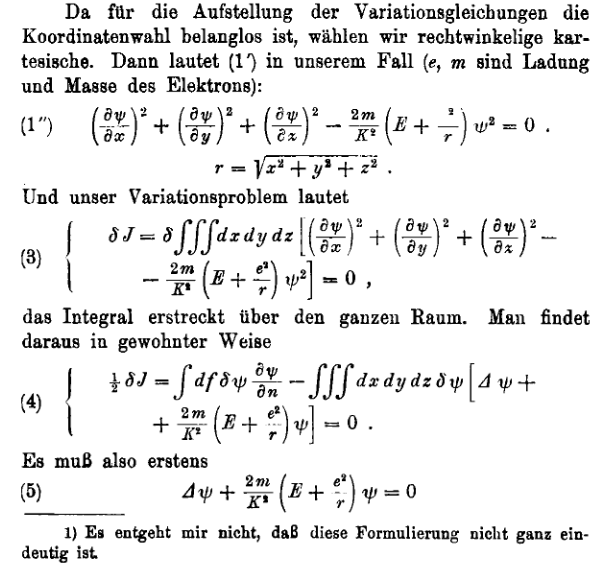
\includegraphics[width=0.75\linewidth]{fig/time-inde-schrodinger-eq.png}
    \caption{ส่วนหนึ่งของบทความฉบับแรกที่ตีพิมพ์โดย Erwin Schr\"{o}dinger ในเดือนมกราคมของปี ค.ศ. 1926 โดยเสนอสมการ Time-independent Schr\"{o}dinger Equation (สมการที่ (1") และ (5))}
    \label{fig:schrodinger_paper_1}
\end{figure}
%
\begin{figure}[H]
    \centering
    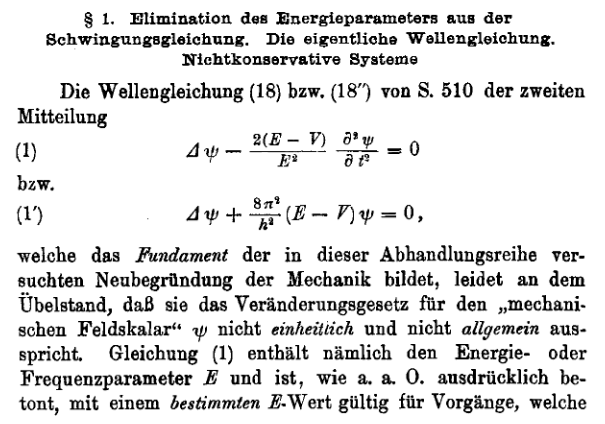
\includegraphics[width=0.75\linewidth]{fig/time-dep-schrodinger-eq.png}
    \caption{ส่วนหนึ่งของบทความฉบับที่ 4 ที่ตีพิมพ์โดย Erwin Schr\"{o}dinger โดยเสนอสมการ Time-dependent Schr\"{o}dinger Equation}
    \label{fig:schrodinger_paper_4}
\end{figure}

สมการชโรดิงเงอร์สามารถแบ่งออกได้เป็นสองแบบคือแบบที่ไม่ขึ้นกับเวลาและแบบที่ขึ้นกับเวลา ดังนี้

\noindent $\bullet$ \textbf{1. Time-independent Schr\"{o}dinger Equation}

\fbox{%
    \begin{minipage}{0.9\linewidth}
        \begin{equation}\label{eq:tise}
            \hat{H} \Psi = E \Psi
        \end{equation}
    \end{minipage}}

\noindent $\bullet$ \textbf{2. Time-dependent Schr\"{o}dinger Equation}

\fbox{%
    \begin{minipage}{0.9\linewidth}
        \begin{equation}\label{eq:tdse}
            i \hbar \frac{d}{d t} \Psi(t) = \hat{H} \Psi(t)
        \end{equation}
    \end{minipage}}

โดย Wavefunction $\Psi(t)$ ที่เป็นฟังก์ชันไอเกน (Eigenfunction) นั้นจะบรรจุข้อมูลเชิงอิเล็กทรอนิกส์ทุกอย่างเกี่ยวกับระบบของเราเอาไว้\autocite{szabo1996,cramer2004,jensen2017} ซึ่งระบบในที่นี้ก็คือโมเลกุล โดยสมการข้างต้นเป็นการคำนวณหาพลังงานของระบบโดยใช้ Hamiltonian Operator $(\hat{H})$ ซึ่งเป็น Operator ที่สอดคล้องกับพลังงาน ซึ่งจริง ๆ แล้วค่าไอเกน (Eigenvalue) ของสมการข้างต้น (สมการที่ \eqref{eq:tdse} และ \eqref{eq:tise}) จะเป็นคุณสมบัติของโมเลกุลอะไรก็ได้ ตราบใดที่เราใช้ Operator ที่สอดคล้องกับคุณสมบัตินั้น ๆ
\idxboth{ฟังก์ชันไอเกน}{Eigenfunction}
\idxboth{ค่าไอเกน}{Eigenvalue}

%--------------------------
\subsection{คุณสมบัติของฟังก์ชันคลื่น}
\label{ssec:wavefunc_prop}
\idxboth{ฟังก์ชันคลื่น!คุณสมบัติ}{Wavefunction!Properties}
%--------------------------

ฟังก์ชันคลื่นเชิงอิเล็กทรอนิกส์ที่ได้มาจากผลเฉลยที่ถูกต้องหรือได้มาจากการประมาณค่านั้นจะต้องมีคุณสมบัติต่อไปนี้

\begin{itemize}[topsep=0pt,noitemsep]\setlength\itemsep{0.5em}
    \item ฟังก์ชันมีค่าที่แน่นอนและมีขอบเขต (Be Finite)

    \item ฟังก์ชันมีความต่อเนื่องและหาค่าได้ตลอดทั้งโดเมน (Be Continuous)

    \item มีผลเฉลยเพียงแค่ค่าเดียวเท่านั้นสำหรับโดเมนหนึ่งค่า (Single-valued) กล่าวคือโดเมนหรืออินพุต $x$ จะต้องให้เรนจ์หรือเอาต์พุต $y$ แค่หนึ่งค่าเท่านั้น

    \item เป็นฟังก์ชันที่มีคุณสมบัติในการมองอิเล็กตรอนทุก ๆ ตัวเหมือนกัน (Indistinguishability of Electron)

    \item ค่ายกกำลังสองของฟังก์ชันเป็นการกระจายตัวของความน่าจะเป็น

    \item ต้องมีความปฏิสมมาตร (Antisymmetry) กล่าวคืออิเล็กตรอนนั้นคือเฟอร์มิออน (Fermion)\autocite{atkins2010} ดังนั้นฟังก์ชันคลื่นจะต้องเปลี่ยนมีการเปลี่ยนเครื่องหมายเมื่ออิเล็กตรอนสองตัวใด ๆ มีการแลกเปลี่ยนพิกัดเชิงพื้นที่หรือพิกัดเชิงสปินกัน
\end{itemize}

ถ้าฟังก์ชันนั้นไม่มีคุณสมบัติข้างต้นนี้จะถือว่าไม่มีความเหมาะสมในการนำมาใช้งานและจะให้ผลการคำนวณที่ผิดพลาด

%--------------------------
\section{แฮมิลโทเนียน}
\label{sec:hamiltonian}
%--------------------------

Hamiltonian เป็นสิ่งที่สำคัญมากในเคมีควอนตัมเพราะเปรียบเสมือนเป็นกุญแจที่สามารถไขรหัสหาคำตอบหรือความลับจาก Wavefunction ได้ โดย Hamiltonian Operator ที่เรานำมาใช้งานนั้นจริง ๆ แล้วก็คือ Operator สำหรับการหาพลังงานรวมนั่นเอง โดยเป็นผลรวมของ Operator พลังงานจลน์และพลังงานศักย์
\idxen{Operator}
\idxboth{แฮมิลโทเนียน}{Hamiltonian}

\begin{equation}\label{eq:hamil}
    \hat{H} = \hat{T} + \hat{V}
\end{equation}

\noindent โดยที่พลังงานจลน์นั้นสามารถเขียนให้อยู่ในรูปของ Momentum Operator ได้โดยพิสูจน์จากพลังงานจลน์ในกรณีแบบดั้งเดิม ดังนี้
\idxboth{โมเมนตัม}{Momentum}
\idxboth{พลังงานจลน์}{Kinetic Energy}

\begin{align}
    T & = \frac{1}{2}mv^{2}_{x}   \\
      & = \frac{(mv_{x})^{2}}{2m}
\end{align}

\noindent ทำการจัดรูปใหม่แล้วทำการแทนเทอม $mv_{x}$ ด้วย Momentum Opeator ในทางกลศาสตร์ควอนตัม $(-ih\frac{d}{dx})$ จะได้ Operator ใหม่ดังนี้

\begin{equation}\label{eq:kin_ener_oper}
    \hat{T} = -\frac{\hbar^{2}}{2m}\frac{d^{2}}{dx^{2}}
\end{equation}

สำหรับพลังงานศักย์นั้นตรงไปตรงมา นั่นคือเราสามารถเขียนพลังงานศักย์ในทางควอนตัมได้แบบเดียวกับกรณีกลศาสตร์ดั้งเดิมได้เลย ดังนี้
\idxboth{พลังงานศักย์}{Potential Energy}

\begin{equation}\label{eq:pot_ener_oper}
    \hat{V} = V(x)
\end{equation}

เมื่อเรานำ Operator ของทั้งสองพลังงาน (สมการที่ \eqref{eq:kin_ener_oper} และสมการที่ \eqref{eq:pot_ener_oper}) มารวมกันเราจะได้ Hamiltonian Operator ดังนี้

\begin{equation}
    \hat{H} = -\frac{\hbar^{2}}{2m}\frac{d^{2}}{dx^{2}} + V(x)
\end{equation}

ลำดับต่อมาคือเราจะมาทำการพิจารณาพลังงานศักย์กันก่อนเพราะว่าไม่ซับซ้อนเหมือนกับกรณีของพลังงานจลน์ โดยพลังงานศักย์ที่เราจะพิจารณาก็คือพลังงานงานศักย์คูลอมบ์ (Coulomb Potential Energy หรือ Operator นั่นเอง) โดยมีสมการดังต่อไปนี้ \idxboth{พลังงานงานศักย์!พลังงานคูลอมบ์}{Potential Energy!Coulomb Energy}

\begin{equation}
    E_{q_{1}q_{2}} = q_{1}\frac{q_{2}}{4\pi\epsilon_{0}|\bm{R}|}
\end{equation}

โดยเมื่อเราพิจารณาระบบง่าย ๆ เช่น อะตอมไฮโดรเจนซึ่งมี 1 อิเล็กตรอนและ 1 นิวเคลียส แล้วกำหนดจุดกำเนิด (Origin Point) ซึ่งมีระยะห่างจากอิเล็กตรอนเท่ากับ $แผ่{r}$ หน่วยและมีระยะห่างจากนิวเคลียสเท่ากับ $\bm{R}$ หน่วย จะได้ว่าระยะห่างระหว่างอิเล็กตรอนและนิวเคลียสคือ $\bm{r}-\bm{R}$ หน่วย ดังนั้นเราสามารถเขียน Hamiltonian Operator ได้ดังนี้

\begin{multline}\label{eq:hamil_hydrogen}
    \hat{H} = -\underbrace{\frac{\hbar^{2}}{2M} \left( \pdv[2]{X} + \pdv[2]{Y} + \pdv[2]{Z} \right)}_{\text{Nuclear Kinetic Energy}}
    \\
    -\underbrace{\frac{\hbar^{2}}{2m} \left( \pdv[2]{x} + \pdv[2]{y} + \pdv[2]{z} \right)}_{\text{Electronic Kinetic Energy}}
    \\
    -\underbrace{\frac{1}{4\pi\epsilon_{0}}\frac{e^{2}}{|\bm{r}-\bm{R}|}}_{\text{Electron-Nucleus Attraction}}
\end{multline}

\noindent โดยเราสามารถใช้สัญลักษณ์ $\nabla^{2}$ หรือ Laplace Operator ($\nabla$ อ่านว่า Nabla) ซึ่งเป็นอนุพันธ์อันดับที่สองของพลังงานจลน์ของนิวเคลียส (เทอมแรก) และของพลังงานจลน์ของอิเล็กตรอน (เทอมที่สอง) ของสมการที่ \eqref{eq:hamil_hydrogen} โดยสามารถเขียนสมการใหม่ได้ดังนี้

\begin{equation}\label{eq:hamil_reduced}
    \hat{H} 
    = 
    -\frac{\hbar^{2}}{2M} \nabla^{2}_{\bm{R}} - \frac{\hbar^{2}}{2m} \nabla^{2}_{\bm{r}}
    -\frac{1}{4\pi\epsilon_{0}}\frac{e^{2}}{|\bm{r}-\bm{R}|}
\end{equation}

ถึงแม้ว่าสมการที่ \eqref{eq:hamil_reduced} มีความเรียบง่ายแล้วแต่ว่าในเคมีควอนตัมนั้นเราจะไม่ได้ใช้สมการของ Operator ที่อยู่ในหน่วย SI (SI Units) โดยนักเคมีทฤษฎีนั้นจะใช้หน่วยอะตอม (Atomic Units หรือย่อได้เป็น a.u. หรือบางครั้งก็เขียนแค่ au)\footnote{อ่านรายละเอียดเกี่ยวกับ Atomic Units ได้ที่ \url{https://en.wikipedia.org/wiki/Hartree_atomic_units}} ซึ่งเมื่อเราเขียนสมการในรูปของ Atomic Units แล้วจะได้สมการที่เรียบง่ายกว่าเดิม ดังนี้

\begin{equation}\label{eq:hamil_au}
    \hat{H} = -\frac{1}{2M} \nabla^{2}_{\bm{R}}
    -\frac{1}{2} \nabla^{2}_{\bm{r}}
    -\frac{1}{|\bm{r}-\bm{R}|}
\end{equation}

\noindent โดยจะสังเกตได้ว่าตัวแปรที่เกี่ยวข้องกับอิเล็กตรอนนั้นจะถูกลดรูปไป ปริมาณที่กำหนดให้มีหน่วยเป็น Atomic Units ได้มีดังนี้
\idxen{Atomic Units}
\idxen{SI Units}

\begin{table}[H]
    \centering
    \caption{เปรียบเทียบปริมาณทางเคมีควอนตัมในหน่วย Atomic Units และ SI Units}
    \label{tab:atomic_units}
    \begin{tabular}{lll}\toprule
        \textbf{ปริมาณ} & \textbf{Atomic Units}             & \textbf{ค่าตาม SI Units}      \\\midrule
        พลังงาน         & $\hbar^{2}/m_{e}a_{0}$ (Hartree) & $4.36 \times 10^{-18} J$  \\
        ประจุ           & $e$                              & $1.60 \times 10^{-19} C$  \\
        ความยาว        & $a_{0}$                          & $5.29 \times 10^{-11} m$  \\
        มวล            & $m_{e}$                          & $9.11 \times 10^{-31} kg$ \\
        \bottomrule
    \end{tabular}
\end{table}

สำหรับกรณีของระบบที่มีอิเล็กตรอนมากกว่าหนึ่งตัว เช่น อะตอมฮีเลียมที่มี 2 อิเล็กตรอน เราสามารถกระจายเทอมของ Hamiltonian ได้ดังนี้

\begin{multline}\label{eq:hamil_he_au}
    \hat{H} = -\frac{1}{2M} \nabla^{2}_{\bm{R}}
    -\frac{1}{2} \nabla^{2}_{\bm{r_{1}}}
    -\frac{1}{2} \nabla^{2}_{\bm{r_{2}}}
    -\frac{2}{|\bm{r_{1}}-\bm{R}|}
    \\
    -\frac{2}{|\bm{r_{2}}-\bm{R}|}
    +\frac{1}{|\bm{r_{1}}-\bm{r_{1}}|}
\end{multline}

\noindent โดยทั้ง 6 เทอมคือพลังงานจลน์ของนิวเคลียส, พลังงานจลน์ของอิเล็กตรอนตัวที่ 1, พลังงานจลน์ของอิเล็กตรอนตัวที่ 2, แรงดึงดูดระหว่างอิเล็กตรอนตัวที่ 1 และนิวเคลียส, แรงดึงดูดระหว่างอิเล็กตรอนตัวที่ 2 และนิวเคลียส, และแรงผลักระหว่างอิเล็กตรอน ตามลำดับ

นอกจากเราสามารถใช้การประมาณของบอร์น-ออปเพนไฮเมอร์ (Born-Oppenheimer (BO) Approximation) ซึ่งเป็นเทคนิคที่นำมาใช้เพื่อการประมาณว่า Wavefunction ของโมเลกุลนั้นขึ้นอยู่กับตำแหน่งของอิเล็กตรอนเพียงอย่างเดียวและไม่ขึ้นกับตำแหน่งของนิวเคลียสเนื่องจากว่ามวลของนิวเคลียสนั้นเยอะกว่ามวลของอิเล็กตรอนมาก ซึ่งถ้าหากใช้ BO Approximation กับ Hamiltonian ของอะตอมฮีเลียมนั้น เทอมแรกของสมการที่ \eqref{eq:hamil_he_au} จะไม่ถูกนำมาพิจารณาในการคำนวณพลังงานของระบบ
\idxboth{การประมาณของบอร์น-ออปเพนไฮเมอร์}{Born-Oppenheimer Approximation}

%--------------------------
\section{การแก้สมการฟังก์ชันคลื่นเพื่อคำนวณพลังงาน}
\label{sec:wavefunc_ener}
%--------------------------

\begin{figure}[H]
    \centering
    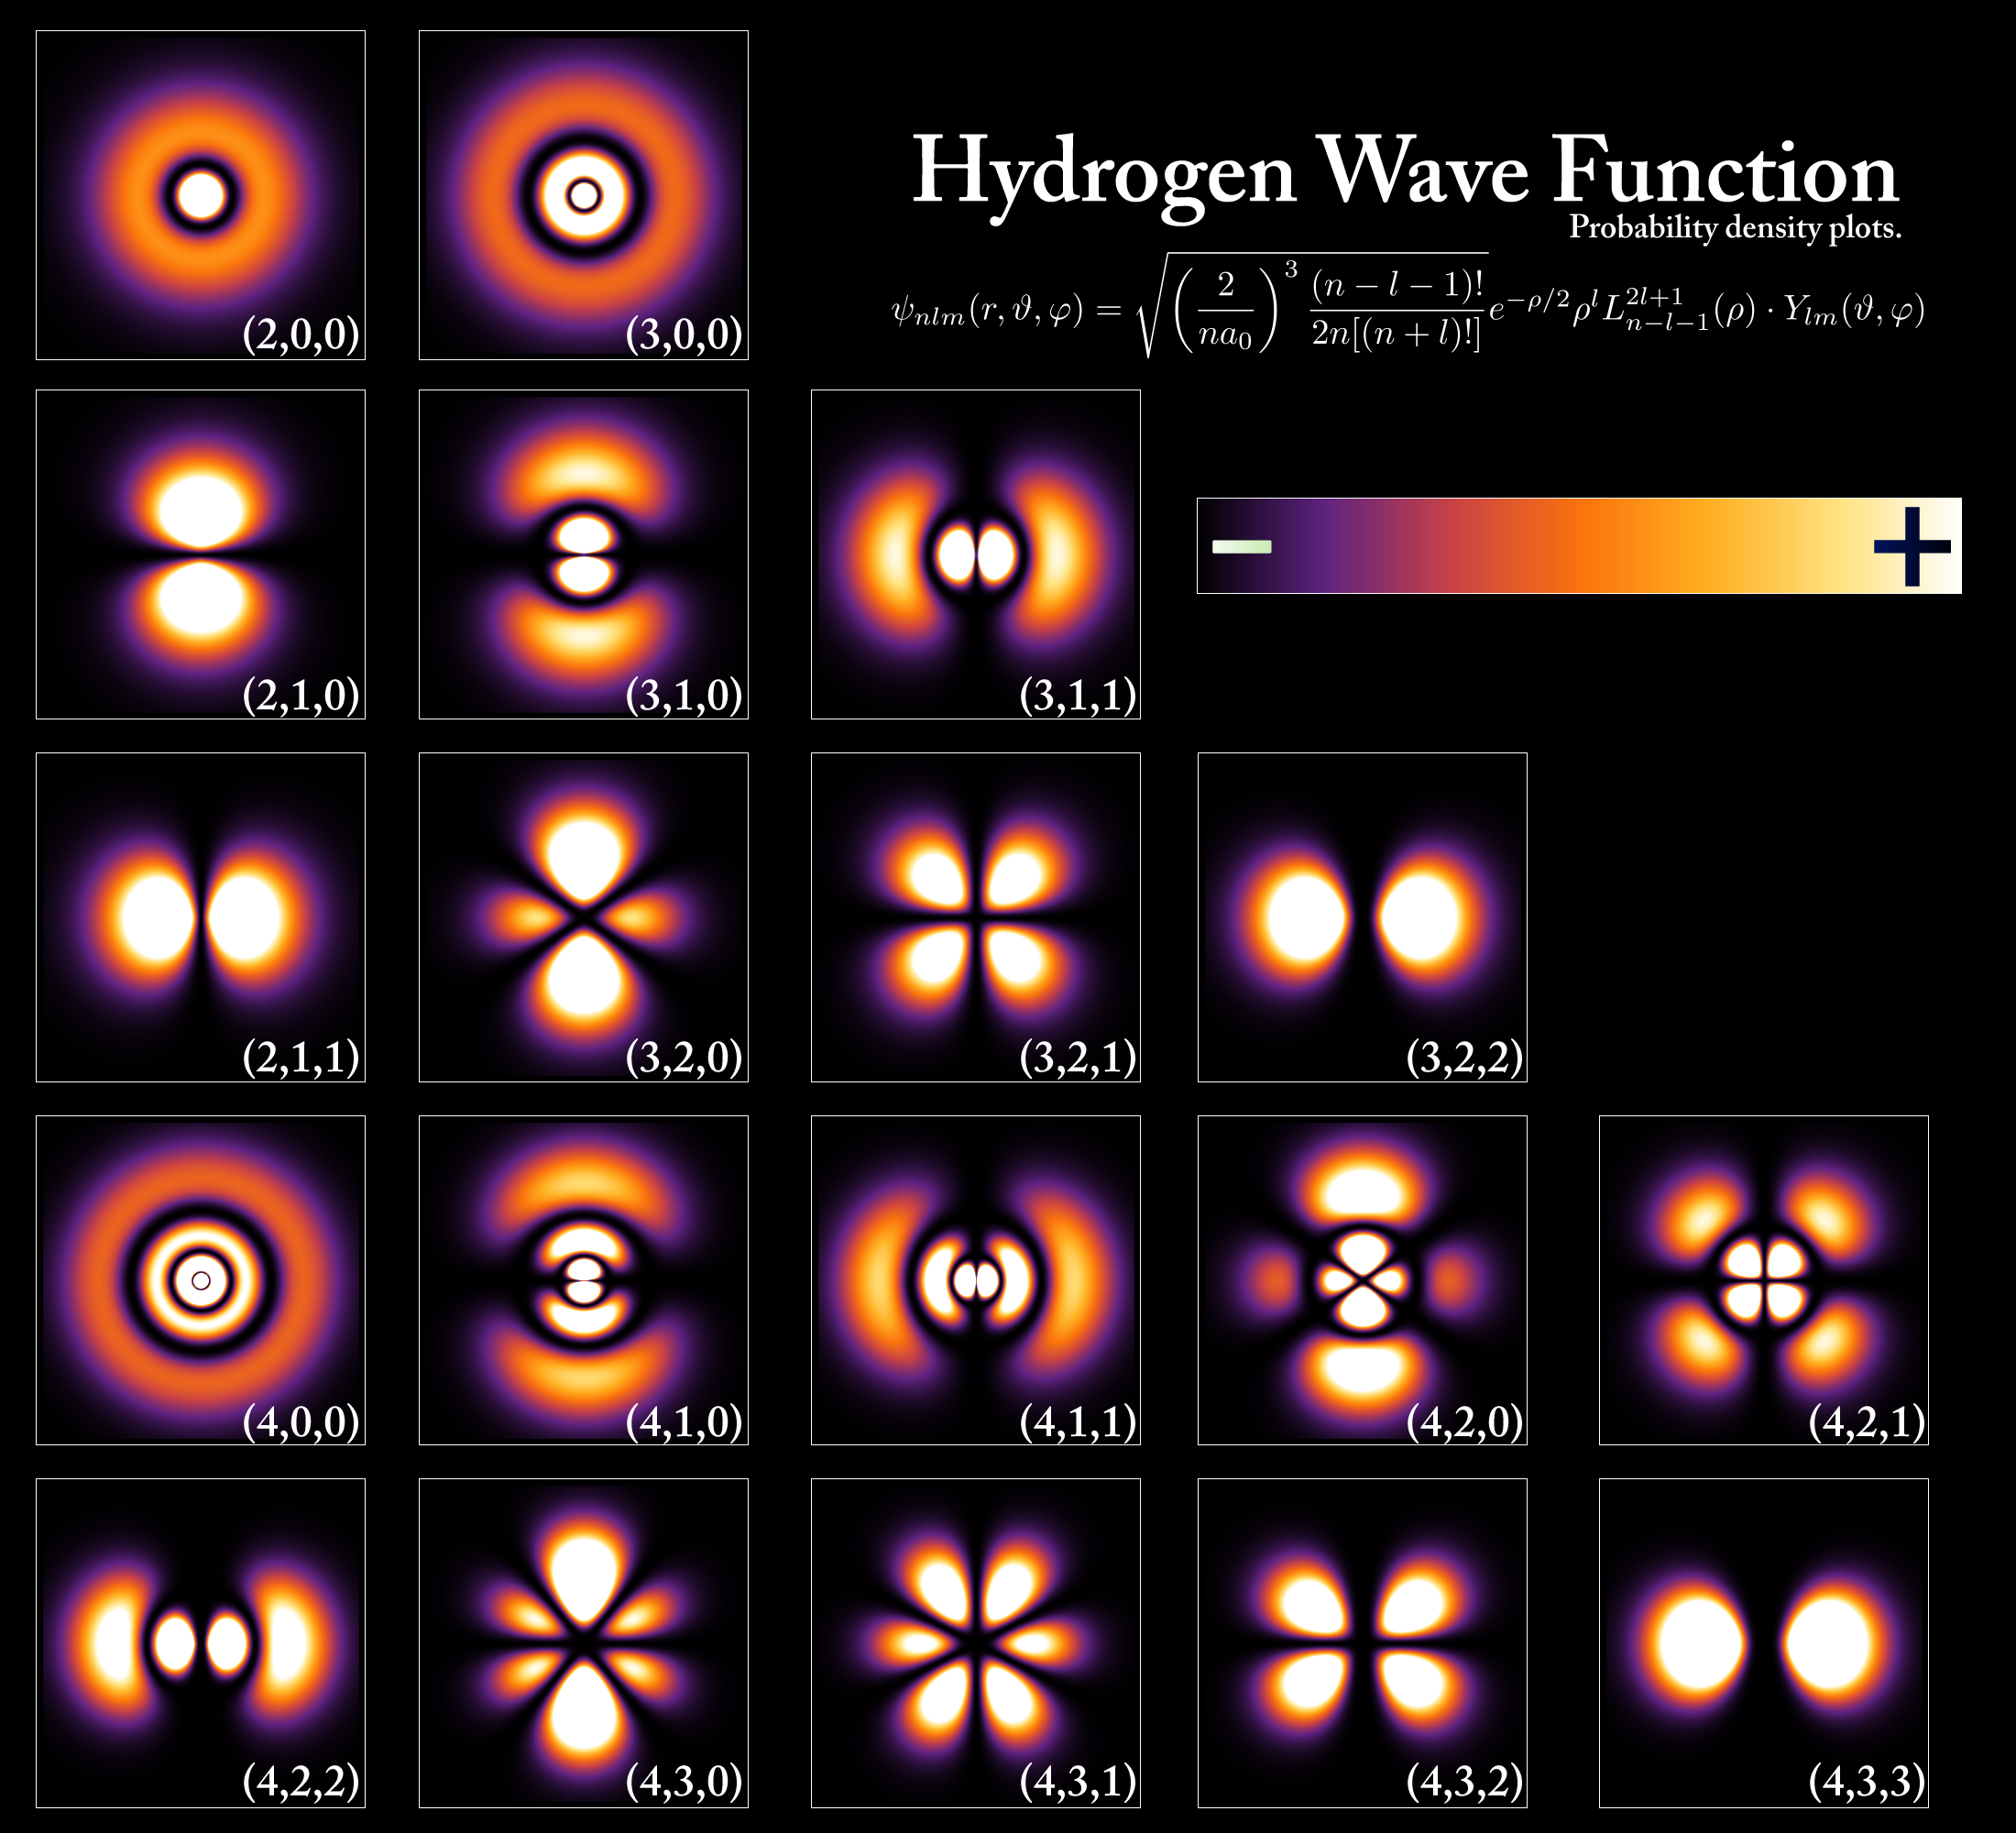
\includegraphics[width=0.8\linewidth]{fig/hydrogen_density_plots.png}
    \caption{แบบจำลองของออร์บิทัลเชิงอะตอม (Atomic Orbitals) ของอิเล็กตรอนของอะตอมไฮโดรเจนที่ระดับพลังงานที่แตกต่างกัน โดยความเข้มของสีที่ไฮไลท์บ่งบอกถึงโอกาสที่จะพบอิเล็กตรอน ณ ตำแหน่งนั้น (เครดิตภาพ: \url{https://en.wikipedia.org/wiki/Atomic_orbital})}
    \label{fig:hydrogen_density}
\end{figure}

หนึ่งในเป้าหมายสำคัญของกลศาสตร์ควอนตัมเชิงโมเลกุล (Molecular Quantum Mechanics) ก็คือการหาวิธีแก้สมการ Time-independent Schr\"{o}dinger Equation เพื่อให้ได้มาซึ่งคำตอบหรือผลเฉลยที่แม่นยำมากที่สุด ซึ่งจะช่วยให้นักเคมีคำนวณสามารถคำนวณคุณสมบัติโครงสร้างเชิงอิเล็กทรอนิกส์ (Electronic Structure) ของโมเลกุล โดยหัวข้อแรกของบทนี้ที่เราจะมาดูกันแบบละเอียดก็คือการใช้เทคนิคควอนตัมเชิงคำนวณและอาศัยการประมาณค่าในการแก้สมการดังกล่าว โดยทั่วไปนั้นจะมีวิธีการหลัก ๆ 2 วิธีที่สามารถช่วยให้เราหาคำตอบของสมการชโรดิงเงอร์ ได้นั่นคือ \textbf{\textit{ab initio} method} ซึ่งเป็นวิธีที่ความแม่นยำของผลลัพธ์ที่ได้จากการแก้สมการนั้นจะขึ้นอยู่กับโมเดลที่เรานำมาใช้ในการอธิบาย Wavefunction ของระบบของเรา (โมเลกุลจะถูกมองเป็น Many-body System) วิธี \textit{ab initio} ที่ได้มีการพัฒนากันมาตั้งแต่อดีตจนถึงปัจจุบันนั้นมีหลายวิธีมาก\autocite{friesner2005,helgaker2014,jensen2017} วิธีทีได้รับความนิยมมีดังไปนี้
\idxboth{โครงสร้างเชิงอิเล็กทรอนิกส์}{Electronic Structure}

\noindent \textbf{วิธี Hartree-Fock}
%
\begin{itemize}[topsep=0pt,noitemsep]\setlength\itemsep{0.5em}
    \item Hartree-Fock (HF)
    
    \item Restricted open-shell Hartree-Fock (ROHF)
    
    \item Unrestricted Hartree-Fock (UHF)
\end{itemize}

\noindent \textbf{วิธี Post-Hartree-Fock}
%
\begin{itemize}[topsep=0pt,noitemsep]\setlength\itemsep{0.5em}
    \item Møller-Plesset Perturbation Theory (MPn)
    
    \item Configuration Interaction (CI)
    
    \item Coupled Cluster (CC)
    
    \item Quadratic Configuration Interaction (QCI)
    
    \item Quantum Chemistry Composite Methods
\end{itemize}

\noindent \textbf{วิธี Multi-Reference}
%
\begin{itemize}[topsep=0pt,noitemsep]\setlength\itemsep{0.5em}
    \item Multi-Configurational Self-Consistent Field (MCSCF) รวมถึงวิธี CASSCF and RASSCF
    
    \item Multi-Reference Configuration Interaction (MRCI)
    
    \item n-electron Valence State Perturbation Theory (NEVPT)
    
    \item Complete Active Space Perturbation Theory (CASPTn)
    
    \item State Universal Multi-Reference Coupled-cluster Theory (SUMR-CC)
\end{itemize}

นอกจากนี้เป็นที่ทราบกันดีว่าสำหรับโมเลกุลที่มีขนาดใหญ่นั้นการคำนวณด้วยวิธี \textit{ab initio} มีความสิ้นเปลืองสูงมาก (Computationally Expensive)\autocite{grabowski2011} ดังนั้นจึงเป็นที่มาของการพัฒนาวิธีการที่สองนั่นคือ \textbf{Semiempirical method}\autocite{thiel2014,christensen2016,kriz2020} ซึ่งจะใช้แนวคิดในการตีความ Hamiltonian ในรูปแบบที่ง่ายกว่าซึ่งอ้างอิงด้วยออร์บิทัลเชิงโมเลกุล (Molecular Orbital หรือ MO) และอาศัยค่าพารามิเตอร์ที่ได้จากการทดลองเพื่อเพิ่มความแม่นยำ อย่างไรก็ตาม วิธี Density Functional Theory (DFT) ก็ถูกพัฒนาขึ้นมาเพื่อแก้ปัญหาที่เราจะต้องมาแก้หรือประมาณค่า Wavefunction ตรง ๆ ซึ่งทำได้ยากโดยเฉพาะกรณีที่ระบบมีหลายอิเล็กตรอน ดังนั้นในปัจจุบันการคำนวณเชิงควอนตัมส่วนใหญ่จึงเป็นการใช้ DFT เพราะว่ามีความสิ้นเปลืองของการคำนวณที่ต่ำมากเมื่อเทียบกับสองวิธีข้างต้นทีได้กล่าวไปนั่นเอง
\idxboth{วิธีแบบกึ่งการทดลอง}{Semiempirical Method}
\idxboth{ออร์บิทัลเชิงโมเลกุล}{Molecular Orbital}
\idxboth{ทฤษฎีฟังก์ชันนอลความหนาแน่น}{Density Functional Theory}

ตัวอย่างของความสำเร็จในการแก้สมการ Wavefunction ก็คือผลลัพธ์ที่แน่นอนของคุณสมบัติของระบบ กรณีที่เราสามารถหาผลเฉลยได้แน่นอนก็คือระบบที่มีอิเล็กตรอน 1 ตัว ตามแสดงในภาพที่ \ref{fig:hydrogen_density} ซึ่งเป็นแบบจำลองของออร์บิทัลเชิงอะตอม (Atomic Orbital หรือ AO) ของอิเล็กตรอนของอะตอมไฮโดรเจน ผู้อ่านสามารถศึกษาการเขียนโค้ดสำหรับพล็อตออร์บิทัลของอะตอทไฮโดรเจนได้ที่ภาพผนวกหัวข้อที่
\ref{ch:hydro_orbitals}
\idxboth{ออร์บิทัลเชิงอะตอม}{Atomic Orbital}

%--------------------------
\subsection{วิธี Self-Consistent Field}
\label{ssec:scf}
\idxen{Self-Consistent Field}
%--------------------------

ในหัวข้อนี้เราจะมาพูดถึงการแก้สมการชโรดิงเงอร์โดยใช้วิธีที่ชื่อว่า Self-Consistent Field (SCF) ซึ่งเป็นการประมาณค่า Hamiltonian แบบวนซ้ำ (เป็นที่มาของคำว่า \textit{Self-Consistent} ซึ่งมีความหมายประมาณว่าเป็นดำเนินการเปรียบเทียบพารามิเตอร์ใหม่กับพารามิเตอร์เดิมโดยที่ยังคงใช้โมเดลอันเดียวกัน) เริ่มต้นเราจะต้องมาดูกันก่อนว่าการมอง Wavefunction ของระบบหลายอิเล็กตรอนสำหรับวิธี SCF นั้นจะมีการตัดสิ่งที่ซับซ้อนออกไปนั่นก็คืออันตรกิริยาแรงผลักระหว่างอิเล็กตรอน (Electron-electron Repulsion) โดย Wavefunction สามารถถูกอธิบายได้ด้วยสมการชโรดิงเงอร์ที่ไม่ขึ้นกับเวลา ดังต่อไปนี้\autocite{cramer2004}

\begin{equation}\label{eq:tise_elec}
    H^{\circ} \Psi^{\circ} = E^{\circ} \Psi^{\circ}
\end{equation}

โดยกำหนดให้ $H^{\circ} = \sum^{N}_{i=1} h_{i}$ เมื่อ $h$ คือ Hamiltonian สำหรับอิเล็กตรอนตัวที่ $i$ ในระบบที่มีอิเล็กตรอน $N$ ตัว นั่นคือสมการสำหรับระบบที่มีอิเล็กตรอน $N$ ตัวนั้น จะสามารถถูกแยกออกมาได้เป็นสมการของระบบหนึ่งอิเล็กตรอนได้ $N$ สมการและ Wavefunction ของอิเล็กตรอนหนึ่งตัวนั้นจริง ๆ แล้วก็คือออร์บิทัล (Orbital) เราจึงสามารถเขียนสมการของอิเล็กตรอนหนึ่งตัวโดยอ้างอิงจากสมการที่ \eqref{eq:tise_elec} ได้เป็นสมการที่จำเพาะเจาะจงมากขึ้น ดังนี้
\idxboth{ออร์บิทัล}{Orbital}

\begin{equation}\label{eq:tise_elec_i}
    h_{i} \Psi^{\circ}(i) = E^{\circ}_{m} \Psi^{\circ}(i)
\end{equation}

\noindent โดยที่ $E^{\circ}_{m}$ คือพลังงานของอิเล็กตรอนหนึ่งตัวใน MO ซึ่งเขียนแทนด้วย $m$ นั่นเอง สำหรับระบบที่อิเล็กตรอนไม่ขึ้นต่อกัน
\idxboth{ออร์บิทัลเชิงโมเลกุล}{Molecular Orbital}

ด้วยเหตุนี้ Wavefunction รวมของระบบ $(\Psi^{\circ})$ จึงสามารถเขียนให้อยู่ในรูปของ Wavefunction ของอิเล็กตรอนหนึ่งตัวได้ดังนี้

\begin{equation}
    \Psi^{\circ} = \psi^{\circ}_{a}(1) \psi^{\circ}_{b}(1) \dots \psi^{\circ}_{z}(N)
\end{equation}

\noindent ซึ่ง Wavefunction ด้านบนนี้จะขึ้นอยู่กับพิกัดของอิเล็กตรอนทุกตัวและขึ้นกับตำแหน่งของนิวเคลียสหรืออะตอมด้วย\footnote{ตอนนี้เราจะยังไม่พิจารณาสปินของอิเล็กตรอนที่จะต้องสอดคล้องและไม่ขัดกับหลักกีดกันของเพาลี (Pauli Exclusion)     ซึ่งจะมีการรวม Spin-orbital สำหรับ Molecular Orbital $m$ $(\varphi_{m})$ เข้าไปด้วย}
\idxboth{หลักกีดกันของเพาลี}{Pauli Exclusion}

สำหรับกระบวนการหรือขั้นตอนที่เราจะนำมาใช้ในการแก้สมการของระบบอิเล็กตรอนหลายตัวนั้น เราจะพิจารณาสมการรูทฮาน (Roothaan Equation) เป็นหลัก ซึ่งเป็นวิธีหนึ่งในการแก้สมการ Hartree-Fock (HF) ซึ่งมีการกำหนดตัวดำเนินการใหม่ขึ้นมาใช้แทน Hamiltonian นั่นก็คือ Fock Operator โดยที่ Fock Operator $(f_{1})$ ถูกนิยามในเทอมของ Coulomb Operator และ Exchange Operator ขึ้นมา นั่นก็คือ Fock Operator ซึ่งเขียนสมการสำหรับอิเล็กตรอน 1 ตัวได้เป็น

\begin{equation}\label{eq:fock}
    f_{1} \psi_{m}(1) = \varepsilon_{n} \psi_{m}(1)
\end{equation}

%--------------------------
\subsection{สมการ Roothaan}
\label{ssec:roothaan}
\idxen{Roothaan Equation}
%--------------------------

สำหรับการแก้สมการ HF ตรง ๆ โดยใช้ SCF นั้นสามารถทำได้ตรง ๆ ด้วยวิธีการเชิงตัวเลข (Numerical Method) แต่ว่าผลเฉลยที่ได้มานั้นมีความซับซ้อนมาก โดยในเวลาต่อมานักฟิสิกส์และนักเคมีชาวดัตช์ที่ชื่อว่า Clemens C.J. Roothaan จึงได้เสนอวิธีการใหม่สำหรับการอธิบาย MO โดยเรียกวิธีนั้นว่าผลรวมเชิงเส้น (Linear Combination of Atomic Orbitals หรือ LCAO)\autocite{atkins2010} เรามาดูรายละเอียดของ LCAO กันครับ
\idxen{Linear Combination of Atomic Orbitals (LCAO)}

เริ่มต้นเราจะนิยามฟังก์ชันพื้นฐานหรือฟังก์ชันพื้นฐาน (Basis Function) สำหรับระบบที่มีอิเล็กตรอน $N$ ตัวขึ้นมาก่อน ซึ่งเขียนแทนด้วย $\chi_{o}$ ซึ่งไอเดียตอนนี้ก็คือเราจะมองว่า Basis Function แบบที่ง่ายที่สุดที่เราสามารถนำมาใช้ได้นั้นก็คือ AO โดยเราสามารถเขียนฟังก์ชันคลื่นเชิงพื้นที่ (Spatial Wavefunction) ซึ่งเป็น Wavefunction ที่ขึ้นกับตำแหน่งของ AO ให้อยู่ในผลรวมเชิงเส้นของการคูณระหว่างสัมประสิทธิ์เชิงเส้นที่เรายังไม่ทราบค่า $(c_{om})$ กับ Basis Function $\chi_{o}$ ได้ดังนี้
\idxth{ฟังก์ชันพื้นฐาน}
\idxth{ฟังก์ชันพื้นฐาน}
\idxen{Basis Function}
\idxboth{ออร์บิทัลเชิงอะตอม}{Atomic Orbital}
\idxboth{ฟังก์ชันคลื่นเชิงพื้นที่}{Spatial Wavefunction}
\idxboth{สัมประสิทธิ์ที่ยังไม่ทราบค่า}{Unknown Coefficients}

\begin{equation}\label{eq:lcao}
    \psi_{m} = \sum^{N_{o}}_{o=1} c_{om} \chi_{o}
\end{equation}

\noindent เมื่อเราแทนสมการ \eqref{eq:lcao} เข้าไปในสมการ \eqref{eq:fock} เราจะได้

\begin{equation}\label{eq:lcao_in_fock}
    f_{1} \sum^{N_{o}}_{o=1} \chi_{o}(1) = \varepsilon \sum^{N_{o}}_{o=1} c_{om} \chi_{o}(1)
\end{equation}

\noindent แล้วทำการคูณสมการ \eqref{eq:lcao_in_fock} ทั้งสองข้างด้วย $\chi^{*}_{o}(1)$ และทำการอินทิเกรตทั่วทั้ง Space ซึ่งจะทำให้เราได้ความสัมพันธ์ต่อไปนี้

\begin{equation}\label{eq:lcao_in_fock_int}
    \sum^{N_{o}}_{o=1} c_{om} \int \chi^{*}_{o}(1) f_{1} \chi_{o}(1) d\tau_{1} =
    \varepsilon_{m} \sum^{N_{o}}_{o=1} c_{om} \int \chi^{*}_{o}(1) \chi_{o}(1) d\tau_{1}
\end{equation}

\noindent จากสมการข้างต้นเราจะพบว่าจะมีผลคูณของ Basis Function ทั้งสองฝั่ง โดยทางฝั่งซ้ายนั้นเราสามารถนิยามเมทริกซ์ฟ็อกก์หรือ Fock Matrix $(F)$ ได้

\begin{equation}\label{eq:matrix_fock}
    F_{o'o} = \int \chi^{*}_{o'}(1) f_{1} \chi_{o}(1) d\tau_{1}
\end{equation}

\noindent และทางฝั่งขวา เรานิยามสิ่งที่เรียกว่าเมทริกซ์ซ้อนทับหรือ Overlap Matrix $(S)$ ซึ่งเป็นเมทริกซ์ที่อธิบายถึงการซ้อนทับกันระหว่างสถานะ 2 สถานะ
\idxboth{เมทริกซ์ซ้อนทับ}{Overlap Matrix}

\begin{equation}\label{eq:matrix_overlap}
    S_{o'o} = \int \chi^{*}_{o'}(1) \chi_{o}(1) d\tau_{1}
\end{equation}

\noindent ซึ่งเราสามารถเขียนสมการ \eqref{eq:lcao_in_fock_int} ให้อยู่ในรูปของสมการที่เรียกว่า Roothaan Equation ได้กระชับ ๆ ดังนี้

\begin{equation}\label{eq:roothaan}
    F c = \varepsilon S c
\end{equation}

\noindent โดยที่ $c$ คือเมทริกซ์ขนาด $N_{o} \times N_{o}$ ซึ่งประกอบไปด้วยสมาชิกของ Coefficient $c_{om}$ และ $\varepsilon$ คือเมทริกซ์ที่มีขนาด $N_{o} \times N_{o}$ เช่นเดียวกันซึ่งเป็นเมทริกซ์แบบ Diagonal Matrix (สมาชิกที่ไม่ใช่แนวทแยงมีค่าเป็น 0 ทั้งหมด) ซึ่งก็คือพลังงานของ Orbital นั่นเอง ซึ่งตรงจุดนี้เราต้องไม่ลืมว่า Fock Operator $(f_{1})$ นั้นถูกกำหนดให้อยู่ในรูปของ Integral บน MO และขึ้นอยู่กับค่าของ Coefficient $c_{om}$ ด้วย

สำหรับการแก้สมการ \eqref{eq:roothaan} นั้นสามารถทำได้ผ่าน Determinant ดังนี้

\begin{equation}\label{eq:scf_secular}
    det|F - \varepsilon S| = 0
\end{equation}

\noindent เนื่องจากว่าสมการที่ \eqref{eq:scf_secular} นั้นไม่สามารถถูกแก้ได้แบบตรงไปตรงมาเพราะว่าสมาชิกของเมทริกซ์ $F_{o'o}$ นั้นเกี่ยวเนื่องโดยตรงกับ Integral ของ Coulomb Operator และ Exchange Operator ซึ่งขึ้นอยู่กับ Spatial Wavefunction ดังนั้นจึงทำให้การแก้สมการที่ \eqref{eq:scf_secular} นั้นเป็นปัญหาแบบงูกินหาง อย่างไรก็ตามเราสามารถใช้กระบวนการวนซ้ำ (Iterative Method) ในการแก้สมการนี้ (เรียกว่าเป็นการประมาณค่าก็ได้) จนกว่าคำตอบหรือผลลัพธ์ที่เราต้องการ (พลังงาน) จากสมการนั้นลู่เข้า
\idxboth{โอเปอเรเตอร์คูลอมป์}{Coulomb Operator}
\idxboth{โอเปอเรเตอร์แลกเปลี่ยน}{Exchange Operators}
\idxboth{ฟังก์ชันคลื่นเชิงพื้นที่}{Spatial Wavefunction}

%--------------------------
\subsection{การแก้สมการ Roothaan ด้วย Self-Consistent Field}
\label{ssec:roothaan_scf}
%--------------------------

\begin{figure}[H]
    \centering
    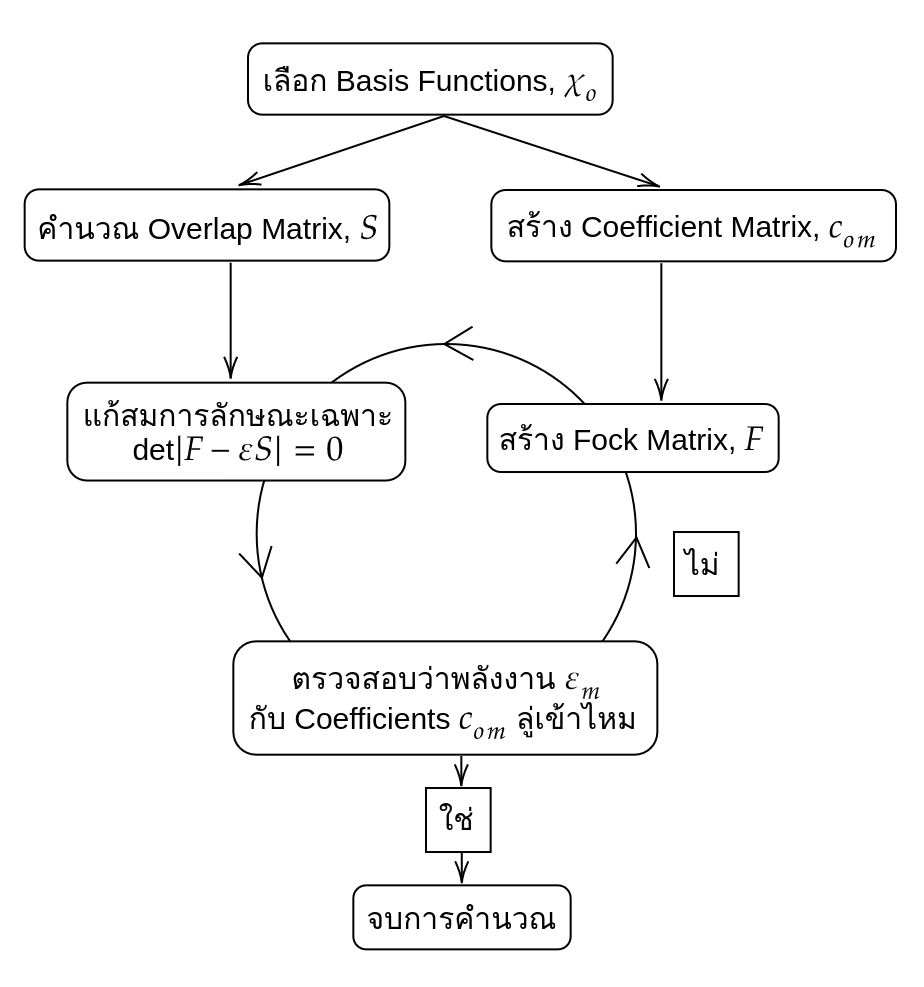
\includegraphics[width=0.75\linewidth]{fig/scf.png}
    \caption{แผนผังขั้นตอนของการประมาณค่าหาพลังงานของออร์บิทัลด้วยวิธี SCF}
    \label{fig:scf}
\end{figure}

ภาพที่ \ref{fig:scf} แสดงแผนผังอัลกอริทึมของวิธี SCF โดยเริ่มจากการเลือก Atomic Basis Function ซึ่งถือว่าเป็นองค์ประกอบหลักของการนำไปสร้าง (Formulate) $S$ โดยใช้สมการ \eqref{eq:matrix_overlap} กับ $c_{om}$ ซึ่งเราจะใช้วิธีการสร้างค่าเริ่มต้นด้วยวิธี Guess ซึ่งมีด้วยกันหลายวิธี เช่น
%
\begin{enumerate}[topsep=0pt,noitemsep]\setlength\itemsep{0.5em}
    \item \textbf{H{\"u}ckel guess} : ใช้ H{\"u}ckel Orbital\autocite{jensen2017}

    \item \textbf{Superposition of Atomic Densities (SAD)} : ใช้ผลรวมของ Atomic Density ในการสร้าง Density Matrix

    \item \textbf{Generalized Wolfsberg-Helmholtz (GWH)} : เป็นวิธีการที่อาศัย H{\"u}ckel Theory โดยการใช้ Overlap Matrix และ Core Hamiltonian\autocite{wolfsberg1952}

    \item \textbf{CORE} : ทำการทำ Core Hamiltonian ให้เกิดเมทริกซ์รูปทแยง (Diagonalization)

    \item \textbf{Harris} : ใช้ Harris Functional ซึ่งเป็น Non-Self-Consistent Approximation สำหรับ Kohn-Sham Orbital\autocite{harris1985}
\end{enumerate}

ซึ่งโปรแกรมเคมีเชิงคำนวณต่างก็มีการเลือกใช้ Guess Method สำหรับการเดา Coefficient หรือ Wavefunction เริ่มต้นในการแก้ SCF แตกต่างกันไป โปรแกรม Gaussian ใช้วิธี Harris สำหรับการคำนวณ HF และ DFT และใช้ H{\"u}ckel หรือ CORE สำหรับ Semiempirical Methods, โปรแกรม Q-Chem และ Psi4 ใช้วิธี SAD กับ GWH เป็นวิธีเริ่มต้นโดยอัตโนมัติ เป็นต้น

หลังจากสร้าง Coefficient Matrix ขั้นตอนต่อไปคือการสร้าง Fock Matrix $(F)$ โดยใช้สมการ \eqref{eq:matrix_fock} หลังจากนั้นเราจะทำการแก้สมการลักษณะเฉพาะ (Secular Equation) สมการที่ \eqref{eq:scf_secular} เพื่อหา Energy Matrix แล้วก็ทำการวนซ้ำขั้นตอนการสร้าง $S$ กับ $F$ ไปปรับหาค่าพลังงานไปเรื่อย ๆ จนกว่าค่าความคลาดเคลื่อนหรือ Error จะมีค่าน้อยกว่าค่าที่กำหนดไว้ (Threshold) แล้วจึงสิ้นสุดกระบวนการ SCF เมื่อค่าพลังงานนั้นลู่เข้า

%--------------------------
\subsection{การคำนวณอนุพันธ์ของพลังงานและเมทริกซ์เฮสเซียน}
\label{ssec:ener_der}
\idxboth{อนุพันธ์ของพลังงาน}{Energy Derivative}
\idxboth{เมทริกซ์เฮสเซียน}{Hessian Matrix}
%--------------------------

หลังจากที่เราสามารถหาพลังงานเชิงอิเล็กทรอนิกส์ (Electronic Energy) ได้แล้ว ลำดับถัดไปที่เราสามารถคำนวณได้ก็คือคุณสมบัติต่าง ๆ ของโมเลกุล สิ่งแรกที่เราทำได้และถือว่าสำคัญมาก ๆ ในงานวิจัยทางด้านเคมีควอนตัมก็คือการหาโครงสร้างที่เหมาะสมหรือเสถียรที่สุดของโมเลกุลโดยใช้หลักเกณฑ์พลังงานรวมที่ต่ำที่สุด ซึ่งการที่เราทราบโครงสร้างที่เหมาะสมที่สุดนั้นมีประโยชน์อย่างมากเพราะเราสามารถนำผลการคำนวณไปเทียบกับผลจากการทดลองด้วยเทคนิค X-ray Crystallography, Electron Diffractiom, หรือ Microwave Spectroscopy เป็นต้น โดยการหาโครงสร้างที่สภาวะเหมาะสมหรือสมดุล (Equilibrium Structure) นั้นสามารถทำได้โดยหาอนุพันธ์ของพลังงานศักย์ของโมเลกุลเทียบกับพิกัดนิวเคลียร์ ซึ่งวิธีการที่เราสามารถนำมาหาอนุพันธ์เพื่อให้ได้ผลลัพเชิงวิเคราะห์ (Analytical Method) เรียกว่า Gradient Method ซึ่งเร็วและให้ผลลัพธ์ที่แม่นยำกว่าระเบียบวิธีเชิงตัวเลข (Numerical Method)

สำหรับอนุพันธ์ของพลังงานนั้นเราจะเริ่มต้นพิจารณากรณีแบบง่ายก่อนนั่นก็คือโมเลกุลที่มีอะตอมสองอะตอม โดยเราจะเขียนพลังงานศักย์ของโมเลกุลเป็น $E$ ซึ่งจะมีเทอมที่เป็นแรงผลักระหว่างนิวเคลียสของทั้งสองอะตอมด้วย ซึ่งแรงผลักนี้จะขึ้นกับระยะห่างระหว่างนิวเคลียส (Internuclear Distance) หรือ $R$ นอกจากนี้เรายังทราบอีกด้วยว่าสำหรับโครงสร้างที่อยู่ในสมดุลนั้น แรง (Force) ที่กระทำต่อนิวเคลียสโดยอิเล็กตรอนนั้นจะเท่ากับศูนย์ ซึ่งแรงดังกล่าวเป็นแรงย่อยมีนิยามคืออนุพันธ์อันดับที่หนึ่งของพลังงานศักย์เทียบกับพิกัดของนิวเคลียสที่ $i$

\begin{align}
    f_{i} & = - \pdv{E}{q_{i}} \\
          & = 0
\end{align}

โดยการคำนวณหาอนุพันธ์ข้างต้นด้วยวิธีการวิเคราะห์หรือ Analytical Method นั้นเราจะต้องทำการคำนวณหาอนุพันธ์ของอินทิกรัลของอิเล็กตรอนหนึ่งตัวและอิเล็กตรอนสองตัว (One-electron กับ Two-electron Integrals) เทียบกับพิกัดนิวเคลียร์ นั่นคือเราจะต้องทำการหาอนุพันธ์ของ Basis Function นั่นเอง\footnote{Basis Function ก็คือ Basis ที่เกิดขึ้นมาจาก Atomic Orbtials ที่ถูก centered หรือมีตำแหน่ง    อยู่ที่จุดอ้างอิงของนิวเคลียสของอะตอมในโมเลกุล} ซึ่งเราสามารถทำได้ผ่านการใช้กฎลูกโซ่ (Chain Rule) โดยทำการหาอนุพันธ์ของพลังงานศักย์เทียบกับ Expansion Coefficient

ลำดับถัดมาคือการหาเมทริกซ์เฮสเซียน (Hessian Matrix) ซึ่งสามารถทำได้โดยการหาอนุพันธ์ย่อยอันดับที่สองของพลังงานศักย์เทียบกับนิวเคลียสของอะตอมตัวที่ $i$ และ $j$ $(\pdv{E}{q_{i}}{q_{j}})$ ซึ่งช่วยให้เราสามารถระบุได้ว่าค่าพลังงานที่คำนวณออกมาได้นั้นสอดคล้องกับจุดต่ำสุดหรือสูงสุดบนพื้นผิวพลังงานศักย์ (Potential Energy Surface หรือ PES) โดยจะสอดคล้องกับอนุพันธ์อันดับที่สองที่ได้ค่าออกมาเป็นบวก (สำหรับ Minimum Point) และลบ (สำหรับ Maximum Point) ตามลำดับ

%--------------------------
\subsection{จากอนุพันธ์ของพลังงานสู่คุณสมบัติเชิงโมเลกุล}
\label{ssec:ener_der_mol_prop}
\idxboth{อนุพันธ์ของพลังงาน}{Energy Derivative}
\idxboth{คุณสมบัติเชิงโมเลกุล}{Molecular Properties}
%--------------------------

คุณสมบัติเชิงโมเลกุลที่เกี่ยวข้องโครงสร้างเชิงอิเล็กทรอนิกส์นั้นเป็นสิ่งที่สำคัญและจำเป็นมากในการคำนวณทางด้านเคมีควอนตัม เพราะว่าคุณสมบัติหรือปริมาณเหล่านี้เป็นสิ่งที่เรานำไปใช้ในการศึกษาโมเลกุลและปฏิกิริยาเคมี แล้วเราสามารถนำผลการคำนวณไปเปรียบเทียบกับค่าที่วัดได้จากการทดลองเพื่อตรวจสอบและยืนยันความถูกต้องของทฤษฎีที่ใช้ในการคำนวณคุณสมบัตินั้น ๆ ด้วย ตามที่ได้อธิบายไปก่อนหน้านี้ว่าอนุพันธ์ของพลังงานนั้นเปรียบเสมือนเป็นกุญแจที่สามารถนำไปไขกล่องที่เก็บซ่อนความลับของโมเลกุลได้ โดยเราสามารถแบ่งความสำคัญของคุณบัติเชิงโมเลกุลออกได้เป็น 3 ประเภท ดังนี้
%
\begin{enumerate}[topsep=0pt,noitemsep]\setlength\itemsep{0.5em}
    \item ความแตกต่างของพลังงาน (Energy Differences) เช่น พลังงานของปฏิกิริยา (Reaction Energies), พลังงานในการทำให้กลายเป็นอะตอม (Atomization Energies), พลังงานที่ใช้ในการสลายโมเลกุล (Dissociation Energies), พลังงานที่แตกต่างกัน          ระหว่างคอนฟอร์เมอร์หรือไอโซเมอร์

    \item คุณสมบัติเชิงโมเลกุลสำหรับสถานะเชิงอิเล็กทรอนิกส์ เช่น โครงสร้าง ณ สภาวะสมดุล (Equilibrium Structure), ไดโพลโมเมนต์ (Dipole Moment), ความสามารถในการมีสภาพขั้ว (Polarizability), ความถี่เชิงการสั่น (Vibrational Frequencies), ความสามารถในการมีสภาพแม่เหล็ก (Magnetazibility), NMR Chemical Shifts

    \item คุณสมบัติที่บ่งบอกการทรานซิชั่นระหว่างสถานะเชิงอิเล็กทรอนิกส์ที่แตกต่างกันได้ เช่น พลังงานกระตุ้นเชิงอิเล็กทรอนิกส์ (Electronic Excitation Energies), ความเข้มของการทรานซิชั่นของโฟตอน 1 ตัวและ 2 ตัว (One- and two-photon Transition Strengths), ระยะเวลาชีวิตในการแผ่รังสี (Radiative Life Times), พลังงานศักย์ในการทำให้เกิดไอออน (Ionization Potentials)
\end{enumerate}

โดยในหัวข้อนี้เราจะสนใจคุณสมบัติเชิงโมเลกุลประเภทที่ 2 ซึ่งเกี่ยวกับสถานะเชิงอิเล็กทรอนิกส์เป็นพิเศษ โดยต้องเกริ่นก่อนว่าคุณสมบัติเชิงโมเลกุลนั้นเกิดขึ้นจากการที่โมเลกุลมีการตอบสนอง (Response) ต่อสนาม (Field) ที่กระทำต่อโมเลกุลซึ่งมองได้ในรูปของอนุพันธ์อันดับต่าง ๆ ของพลังงาน เช่น อนุพันธ์สามอันดับแรก ดังนี้
%
\begin{itemize}[topsep=0pt,noitemsep]\setlength\itemsep{0.5em}
    \item อนุพันธ์อันดับหนึ่ง: แรง (Force), ความเครียด (Stress), Dipole Moment เป็นต้น
    \item อนุพันธ์อันดับสอง: Dielectric Susceptibility, Polarizability, Born Effective Charges เป็นต้น
    \item อนุพันธ์อันดับสาม: Nonlinear Dielectric Susceptibility, (First-order) Hyperpolarizability เป็นต้น
\end{itemize}

โดยเราสามารถเขียนพลังงานที่อยู่ภายใต้สนามภายนอก (External Field) ในรูปของฟังก์ชันการกระจายของเทเลอร์ (Taylor Expansion) รอบ ๆ ตำแหน่งที่ไม่มีสนาม (Field-free) ได้ดังนี้
%
\begin{equation}\label{eq:ener_taylor}
    E(\epsilon) = E(\epsilon = 0)
    + \underbrace{\evaluated{\dv{E}{\epsilon}}_{\epsilon = 0} \epsilon}_{\text{First Response}}
    + \underbrace{\frac{1}{2} \evaluated{\dv[2]{E}{\epsilon}}_{\epsilon = 0} \epsilon^{2}}_{\text{Second Response}}
    + \dots
\end{equation}
%
\noindent สำหรับเทอมที่สองที่เป็นอนุพันธ์อันดับสองของพลังงานนั้นคือ Gradient ซึ่งเป็นฟังก์ชันแบบเส้นตรงสำหรับ (Linear) เราจึงเรียกคุณสมบัติที่ได้จากเทอมนี้ว่า Linear Response Properties ส่วนเทอมอื่น ๆ เช่น เทอมที่สามนั้นเป็นอนุพันธ์อันดับสองซึ่งจะเกี่ยวข้องกับฟังก์ชัน Quadratic นอกจากนี้เรายังสามารถสรุปได้ว่า
%
\begin{framed}
    \begin{align*}
         & \text{Dipole Moment}\,(\mu)               &  & = &  & -\evaluated{\dv{E}{\epsilon}}_{\epsilon = 0}    \\
         & \text{Polarizability}\,(\alpha)           &  & = &  & -\evaluated{\dv[2]{E}{\epsilon}}_{\epsilon = 0} \\
         & \text{First Hyperpolarizability}\,(\beta) &  & = &  & -\evaluated{\dv[3]{E}{\epsilon}}_{\epsilon = 0}
    \end{align*}
\end{framed}

โดยเราสามารถคำนวณคุณสมบัติเชิงโมเลกุลต่าง ๆ เหล่านี้ด้วยวิธีการคำนวณทั่วไป เช่น วิธี HF หรือ DFT เพื่อนำไปใช้เป็นลักษณะเฉพาะ (Feature) สำหรับการฝึกสอนโมเดล ML หรือนำมาใช้เป็นเอาต์พุตสำหรับการทำนายก็ได้

%--------------------------
\section{ทฤษฎีฟังก์ชันนอลความหนาแน่น}
\label{sec:dft}
\idxboth{ทฤษฎีฟังก์ชันนอลความหนาแน่น}{Density Functional Theory}
%--------------------------

ตามที่ผู้เขียนได้พูดถึง \textit{\enquote{ทฤษฎีฟังก์ชันนอลความหนาแน่น}} หรือ \textit{\enquote{Density Functional Theory (DFT)}} ในบทก่อนหน้านี้แล้วว่าเป็นทฤษฎีที่มีความสำคัญมากในวงการวิทยาศาสตร์นั่นก็เพราะว่าทฤษฎี DFT ได้พลิกโฉมงานวิจัยที่เกี่ยวข้องกับการศึกษาโครงสร้างเชิงอิเล็กทรอนิกส์ของโมเลกุลไปอย่างสิ้นเชิง แทนที่จะมองโมเลกุลเป็นระบบที่อิเล็กตรอนมีอันตรกิริยากันตรง ๆ แล้วใช้ Wavefunction ในการอธิบายระบบนั้น วิธี DFT จะมองโมเลกุลว่าเป็นกลุ่มก้อนของอิเล็กตรอนและใช้ความหนาแน่น (Density) ในการอธิบายแทน จึงทำให้เราไม่จำเป็นที่จะต้องแก้สมการเพื่อหาผลเฉลยแบบแม่นตรง (Exact Solution) ของ Wavefunction (ซึ่งเราไม่สามารถคำนวณหาบางเทอมของ Wavefunction ได้สำหรับกรณีที่ระบบมีอิเล็กตรอนมากกว่าหนึ่งตัว)

%--------------------------
\subsection{ฟังก์ชันและฟังก์ชันนอล}
\label{ssec:function_functional}
\idxboth{ฟังก์ชัน}{Function}
\idxboth{ฟังก์ชันนอล}{Functional}
%--------------------------

ก่อนที่ผู้อ่านจะได้ศึกษาในหัวข้อต่อไปซึ่งจะลงรายละเอียดมากกว่านี้ ผู้เขียนขอเริ่มด้วยการอธิบายความหมายและการใช้งานของสิ่งที่เรียกว่าฟังก์ชันและฟังก์ชันนอลก่อนครับ เพราะว่าการที่เราเข้าใจความหมายและความแตกต่างของคำศัพท์สองคำนี้จะเป็นพื้นฐานสำคัญในการเข้าใจทฤษฎี DFT ที่ว่าด้วยเรื่องของความหนาแน่นของอิเล็กตรอนที่ผู้อ่านจะได้ศึกษาในหัวข้อที่ \ref{ssec:elec_density} โดยฟังก์ชันกับฟังก์ชันนอลนั้นต่างกันอินพุต ดังนี้

\begin{description}
    \item[$\bullet$ ฟังก์ชัน (Function)] รับอินพุตที่เป็นตัวเลขและให้เอาต์พุตที่เป็นตัวเลขเช่นเดียวกัน โดยสามารถเขียนการ Mapping ได้เป็น $x_0 \mapsto f(x_0)$ โดยที่ $x_{0}$ คืออาร์กิวเมนต์หรืออินพุตของฟังก์ชัน $f$

        ตัวอย่างของฟังก์ชัน เช่น
        \begin{align*}
            f(x)   & = x^{2}                                \\
            g(x,y) & = \cos(x) + e^{-3\sqrt{x^{2} + y^{2}}}
        \end{align*}

    \item[$\bullet$ ฟังก์ชันนอล (Functional)] เป็นฟังชันก์ชนิดหนึ่งซึ่งรับอินพุตที่เป็นฟังก์ชันและให้เอาต์พุตที่เป็นตัวเลข ซึ่งสรุปได้ง่าย ๆ ว่า \enquote{ฟังก์ชันนอลนั้นก็คือฟังก์ชันของฟังก์ชัน} โดยสามารถเขียนการ Mapping ได้เป็น $f \mapsto f(x_0)$ โดยที่ $x_{0}$ คือพารามิเตอร์

        ตัวอย่างของฟังก์ชันนอล เช่น
        \begin{align*}
            F[f] & = \int^{\infty}_{-\infty} f^{3}(x) \, dx                                                \\
            H[g] & = \int^{3}_{2} \int^{4}_{-10} \left ( \pdv[2]{g(x,y)}{x} - 2.3 g(x,y) \right ) \, dx dy
        \end{align*}
\end{description}

เมื่อทราบความแตกต่างแล้วผู้อ่านก็น่าจะพอเดาออกแล้วว่าคำว่า \enquote{Functional} ในชื่อของทฤษฎี Density Functional Theory นั้นบ่งบอกว่าเป็นทฤษฎีที่อธิบายโครงสร้างเชิงอิเล็กทรอนิกส์ของโมเลกุลด้วยฟังก์ชันนอลที่สามารถอธิบายความหนาแน่นของอิเล็กตรอนได้

%--------------------------
\subsection{จากฟังก์ชันคลื่นสู่ความหนาแน่นเชิงอิเล็กทรอนิกส์}
\label{ssec:elec_density}
\idxboth{ความหนาแน่นเชิงอิเล็กทรอนิกส์}{Electronic Density}
%--------------------------

ในการพิจารณาฟังก์ชันคลื่นของอิเล็กตรอนนั้นเราไม่สามารถพิจารณาแค่พิกัดหรือตำแหน่งของอิเล็กตรอนเชิงพื้นที่ (Spatial Coordinates) หรือ $(x, y, z)$ แต่ยังต้องพิจารณาตำแหน่งของสปิน (Spin Coordinates) หรือ $\omega$ ด้วย ดังนั้นจำนวนตัวแปรที่ส่งผลต่อ Wavefunction จึงมีทั้งหมด 4 ตัวแปรต่อหนึ่งอิเล็กตรอน ถ้าหากระบบของเรามี $N$ อิเล็กตรอน จำนวนตัวแปรของ Wavefunction ก็จะเท่ากับ $4 N_{\text{electrons}}$

เพื่อทำให้ชีวิตง่ายขึ้น แนวคิดในการใช้ความหนาแน่นสำหรับศึกษาโครงสร้างเชิงอิเล็กทรอนิกส์ของโมเลกุลแทนที่จะใช้ Wavefunctionโดยตรงนั้นจึงได้รับความสนใจและถูกพัฒนาเรื่อยมาจนถึงปัจจุบัน ข้อดีของการอธิบายระบบ (โมเลกุล) ด้วยความหนาแน่นแทนที่จะใช้ Wavefunction นั้นช่วยทำให้ลดความสิ้นเปลืองในการคำนวณไปได้เยอะมากเพราะความหนาแน่นนั้นสามารถถูกเขียนด้วยฟังก์ชันที่ขึ้นอยู่กับตัวแปรเพียงแค่ 3 ตัวเท่านั้น (สำหรับกรณีที่ไม่พิจารณาสปินของอิเล็กตรอน) กล่าวคือสำหรับ Wavefunction ที่เขียนด้วย Schr\"{o}dinger Equation นั้นจะเป็นฟังก์ชันที่มีจำนวนมิติคือ $3N_{\text{electron}}$ แต่สำหรับความหนาแน่นนั้นเราจะได้สมการที่มีจำนวนมิติคือ 3 มิติด้วยกันทั้งหมดจำนวน $N$ สมการ (ตามจำนวนอิเล็กตรอน) ซึ่งจะเห็นได้ว่าความซับซ้อนในการคำนวณจะต่างกันอย่างมาก โดยสรุปเป็นความสัมพันธ์ได้ดังนี้

\begin{framed}
    \centering
    $3N$-dimensional Schr\"{o}dinger Equation \\
    $\Psi(\bm{r}_{1}, \bm{r}_{2}, \bm{r}_{3}, \dots, \bm{r}_{N})$ \\
    $\downarrow$ \\
    $N$ $3$-dimensional Single Particle Equation \\
    $n({\bm{r}})$
\end{framed}

\noindent โดยที่ Single Particle Equation ในที่นี้คือสมการที่ใช้ในการอธิบายอนุภาค 1 ตัวซึ่งก็คืออิเล็กตรอนนั่นเอง

จริง ๆ แล้วความหนาแน่นเชิงอิเล็กทรอนิกส์ก็คือความหนาแน่นของอิเล็กตรอน (Electron Density) หรือ $n(\bm{r})$ ซึ่งเป็นหัวใจสำคัญของทฤษฎี DFT เลยก็ว่าได้ โดยความน่าจะเป็นของโอกาสที่จะพบอิเล็กตรอนตัวที่ 1 ของระบบหรือโมเลกุลที่มี $N$ อิเล็กตรอนนั้นสามารถคำนวณได้จากการใช้ปริพันธ์ (Integral) ตามสมการต่อไปนี้

\begin{equation}\label{eq:elec_prob_density_1e}
    P(\bm{1}) = \left [ \int {d}^{3} \bm{r}_{2} \cdots \int {d}^{3} \bm{r}_{N} \,
        \psi^*(\bm{r}_{1}, \bm{r}_{2}, \dots, \bm{r}_{N}) \psi(\bm{r}_{1}, \bm{r}_2,
        \dots, \bm{r}_N) \right ] {d}^{3} \bm{r}_{1}
\end{equation}

เนื่องจากว่าอิเล็กตรอนทุก ๆ ตัวนั้นมีคุณสมบัติเหมือนกันหมดทุกประการ (Indistinguishable) ดังนั้นความหนาแน่นของความน่าจะเป็น (Probability Density) ของอิเล็กตรอนแต่ละตัวก็จะเท่ากันด้วย หมายความว่าความน่าจะเป็นของความหนาแน่นของอิเล็กตรอนตัวที่ 1 ก็เท่ากับของตัวที่ 2, ตัวที่ 3, ไปจนถึงตัวที่ $N$ ดังนั้นในการคำนวณหาความหนาแน่นของความน่าจะเป็น (Probability Density) ของอิเล็กตรอนทั้งหมดนั้นจึงสามารถทำได้โดยการรวมแบบเชิงเส้น นั่นก็คือเราคูณความน่าจะเป็นของโอกาสที่จะพบอิเล็กตรอน 1 ตัวด้วย $N$ นั่นเอง โดยเราจะได้สมการดังนี้
\idxboth{ความหนาแน่นของอิเล็กตรอน}{Electron Density}
\idxboth{ความหนาแน่นของความน่าจะเป็น}{Probability Density}

\begin{equation}\label{eq:elec_density_all}
    n(\bm{r}) = N \underbrace{\int {d}^{3} \bm{r}_{2} \cdots \int {d}^{3} \bm{r}_{N} \,
        \psi^*(\bm{r}, \bm{r}_{2}, \dots, \bm{r}_{N}) \psi(\bm{r}, \bm{r}_2,
        \dots, \bm{r}_N)}_{\textstyle \text{ความน่าจะเป็นที่จะพบอิเล็กตรอน 1 ตัว}}
\end{equation}

\noindent โดยที่ $\psi$ คือฟังก์ชันคลื่นที่ผ่านการถูกทำให้เป็นปกติ (Normalized Wavefunction) มาแล้ว ซึ่งความหมายของการทำให้เป็นปกติ (Normalization) ก็คือการหารูปแบบ (Form) ของ Wavefunction ที่สอดคล้องกับเงื่อนไขดังต่อไปนี้

\begin{equation}\label{eq:square_integrable}
    \int^\infty_{-\infty} \psi^* \psi dx = 1
\end{equation}

อย่างไรก็ตาม ไม่ใช่ทุก Wavefunction ที่สามารถทำ Normalization ได้ ตัวอย่างของฟังก์ชันที่เป็นข้อยกเว้น เช่น Planewave Wavefunction ซึ่งเป็นฟังก์ชันที่ขึ้นกับพิกัดและเวลา ดังนี้ $\psi(x,t) = \psi_0 {\rm e}^{ {\rm i} (k x-\omega t)}$ ไม่เป็น Square-integrable Function

%--------------------------
\subsection{จากความหนาแน่นเชิงอิเล็กทรอนิกส์สู่พลังงานของระบบ}
\label{ssec:ener_density}
\idxen{Density Functional Theory!Electronic Density}
%--------------------------

เมื่อเราเข้าใจนิยามและไอเดียของความหนาแน่นเชิงอิเล็กทรอนิกส์หรือความหนาแน่นของอิเล็กตรอนแล้ว ลำดับต่อไปก็คือเราจะคำนวณพลังงานของระบบ (โมเลกุล) โดยใช้ความหนาแน่นได้อย่างไร ซึ่งตามทฤษฎีนั้นเราสามารถคำนวณพลังงานได้แบบอ้อม ๆ ผ่าน Wavefunction

\begin{figure}[H]
    \centering
    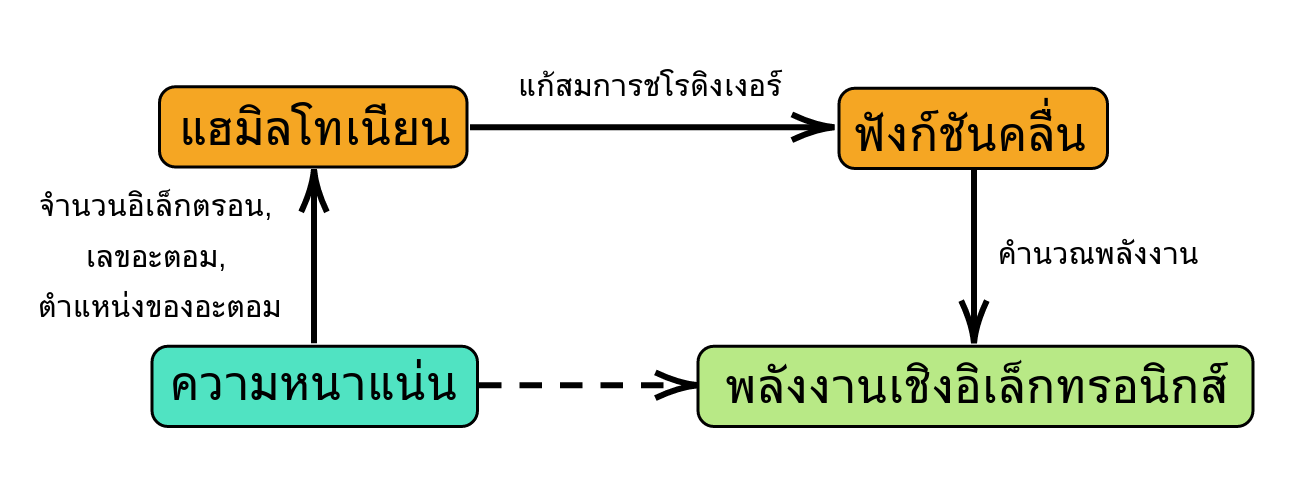
\includegraphics[width=\linewidth]{fig/density_wavefunc_ener.png}
    \caption{ความเชื่อมโยงแบบตรงและแบบอ้อมระหว่างความหนาแน่นของอิเล็กตรอนและพลังงานเชิงอิเล็กทรอนิกส์ของระบบ}
    \label{fig:density_wavefunc_ener}
\end{figure}

จากไดอะแกรมที่แสดงในภาพที่ \ref{fig:density_wavefunc_ener} นั้นสามารถตีความได้ว่าเราสามารถคำนวณพลังงานของระบบโดยผ่าน Hamiltonian และ Wavefunction ได้ซึ่งก็จะมีความซับซ้อนในเชิงคำนวณ ดังนั้นคำถามสำคัญที่ตามมาก็คือ \enquote{จะเป็นไปได้ไหมที่เราจะคำนวณพลังงานจากความหนาแน่นของอิเล็กตรอนตรง ๆ} ซึ่งคำตอบก็คือจริง ๆ แล้วไม่สามารถหาได้ตรง ๆ แต่เรามีทริคที่สามารถทำได้ดังต่อไปนี้

เริ่มจากการกำหนดให้พลังงานเชิงอิเล็กทรอนิกส์ได้จากการคำนวณค่า Expectation Value (ค่าเฉลี่ย) ของ Hamiltonian Operator

\begin{equation}\label{eq:ener_expect_value}
    E_{\text{el}} = \int \cdots \int \Psi^{\ast} \hat{H}_{\text{el}} \Psi \, d\bm{x}_{1} \dots \,
    d\bm{x}_{N_{\text{el}}}
\end{equation}

\noindent โดยที่ Hamiltonian Operator $(\hat{H}_{\text{el}})$ สำหรับอิเล็กตรอนมีสมการดังต่อไปนี้

\begin{equation}\label{eq:hamil_one_elec}
    \hat{H}_{\text{el}} = \sum^{N_{\text{el}}}_{i=1} -\frac{1}{2} \nabla^{2}_{i}
    + \sum^{N_{\text{el}}}_{i=1} \sum^{N_{\text{el}}}_{j=i+1} \frac{1}{|\bm{r}_{i}-\bm{r}_{j}|}
    + \underbrace{\sum^{N_{\text{el}}}_{i=1} \sum^{N_{\text{nu}}}_{A=1} \frac{-Z_{A}}{|\bm{r}_{i}-\bm{R}_{A}|}}    _{\text{Nuclear Attraction Energy}}
\end{equation}

\noindent ซึ่งเทอมที่ 3 ของสมการที่ \eqref{eq:hamil_one_elec} นั้นคือพลังงานดึงดูดระหว่างอิเล็กตรอนกับนิวเคลียสซึ่งมีชื่อเรียกอีกชื่อว่า \enquote{ศักย์ภายนอก} (External Potential) โดยเป็นคำศัพท์ที่ใช้ในทฤษฎี DFT ซึ่งคำว่า External นี้มาจากการที่เราใช้การประมาณของ Born-Oppenheimer ซึ่งเป็นการกำหนดให้นิวเคลียสนั้นเป็นวัตถุที่ถูกตรึงอยู่กับที่ (Fixed) และทำให้เกิดพลังงานศักย์คูลอมป์ (Coulomb Potential) ต่ออิเล็กตรอน ดังนั้นจากสมการที่ \eqref{eq:hamil_one_elec} เราจึงเขียนใหม่ได้เป็น
\idxboth{ศักย์ภายนอก}{External Potential}

\begin{align}\label{eq:hamil_ext_pot}
    \hat{H}_{\text{el}} & = \sum^{N_{\text{el}}}_{i=1} -\frac{1}{2} \nabla^{2}_{i}
    + \sum^{N_{\text{el}}}_{i=1} \sum^{N_{\text{el}}}_{j=i+1} \frac{1}{|\bm{r}_{i}-\bm{r}_{j}|}
    + \sum^{N_{\text{el}}}_{i=1}
    \underbrace{\left ( \sum^{N_{\text{nu}}}_{A=1} \frac{-Z_{A}}{|\bm{r}_{i}-\bm{R}_{A}|} \right )}    _{\text{Nuclear Attraction Energy}} \nonumber                                  \\
                        & = \sum^{N_{\text{el}}}_{i=1} -\frac{1}{2} \nabla^{2}_{i}
    + \sum^{N_{\text{el}}}_{i=1} \sum^{N_{\text{el}}}_{j=i+1} \frac{1}{|\bm{r}_{i}-\bm{r}_{j}|}
    + \sum^{N_{\text{el}}}_{i=1} V_{\text{ext}}(\bm{r}_{i})
\end{align}

\noindent โดยที่มี External Potential $V_{\text{ext}}(\bm{r}_{i})$ กระทำต่ออิเล็กตรอนทุกตัวในโมเลกุล

ลำดับต่อไปก็คือเราลองมาทำการกระจาย Expectation Value ของพลังงานเชิงอิเล็กทรอนิกส์โดยการแทนสมการที่ \eqref{eq:hamil_ext_pot} เข้าไปในสมการที่ \eqref{eq:ener_expect_value} ซึ่งเราจะได้พลังงานที่ประกอบไปด้วย 3 เทอม ดังนี้

\begin{align}\label{eq:ener_express_ext_pot}
    E_{\text{el}} = & \int \cdots \int \Psi^{\ast}
    \left ( \sum^{N_{\text{el}}}_{i=1} -\frac{1}{2} \nabla^{2}_{i} \right )
    \Psi \, d\bm{x}_{1} \dots \, d\bm{x}_{N_{\text{el}}} \nonumber \\
                    & + \int \cdots \int \Psi^{\ast}
    \left ( \sum^{N_{\text{el}}}_{i=1} \sum^{N_{\text{el}}}_{j=i+1} \frac{1}{|\bm{r}_{i}-\bm{r}_{j}|} \right )
    \Psi \, d\bm{x}_{1} \dots \, d\bm{x}_{N_{\text{el}}} \nonumber \\
                    & + \underbrace{\int \cdots \int \Psi^{\ast}
    \left ( \sum^{N_{\text{el}}}_{i=1} V_{\text{ext}}(\bm{r}_{i}) \right )
    \Psi \, d\bm{x}_{1} \dots \, d\bm{x}_{N_{\text{el}}}    }_{\textstyle \int V_{\text{ext}}(\bm{r}) n(\bm{r}) \, d\bm{r}}
\end{align}

\noindent โดยสมการที่ \eqref{eq:ener_express_ext_pot} มีเพียงแค่เทอมที่ 3 เท่านั้นที่สามารถเขียนให้อยู่ในรูปของฟังก์ชันนอลของความหนาแน่นได้ (Explicit Functional of Density)

%--------------------------
\subsection{ความสัมพันธ์ระหว่างความหนาแน่นของอิเล็กตรอนและศักย์ภายนอก}
\label{ssec:ener_density_ext_pot}
%--------------------------

\begin{figure}[H]
    \centering
    \frame{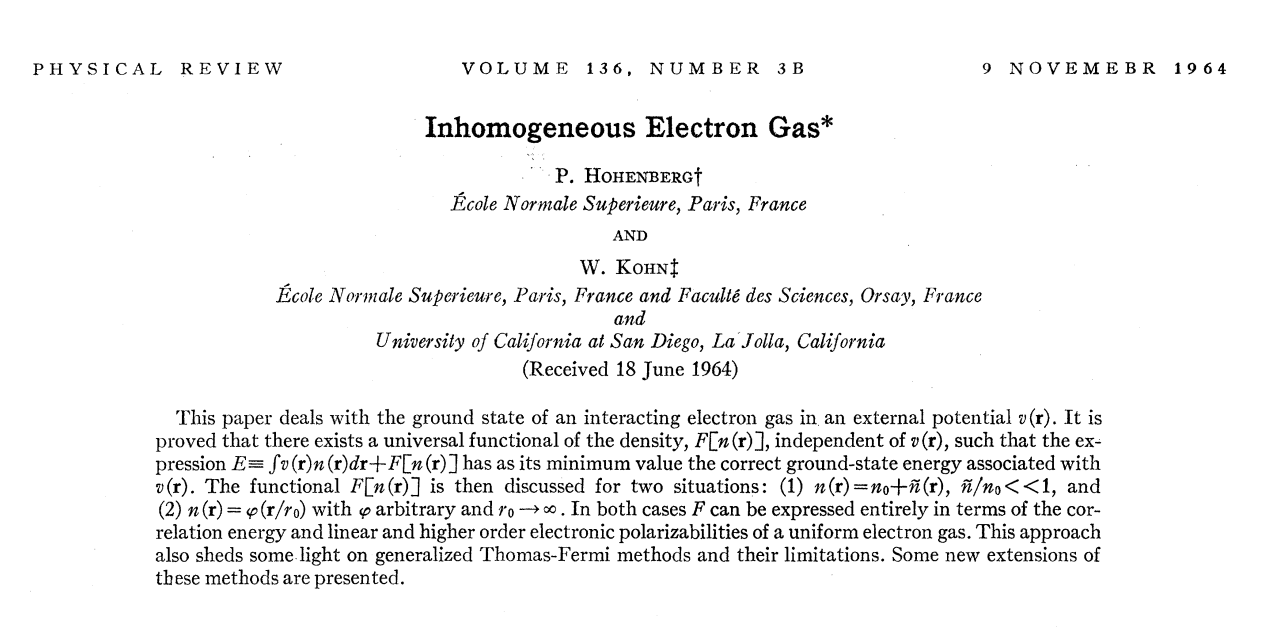
\includegraphics[width=\linewidth]{fig/hohenberg_kohn_abstract.png}}
    \caption{บทคัดย่อของบทความงานวิจัยที่นำเสนอทฤษฎีบท Hohenberg-Kohn ในปี ค.ศ. 1964}
    \label{fig:hohenberg_kohn_abs}
\end{figure}

สำหรับระบบที่มีจำนวนอิเล็กตรอน $N$ ตัวนั้น ศาสตราจารย์ Pierre Hohenberg (New York University) และศาสตราจารย์ Walter Kohn (University of California at Santa Barbara) ได้เสนอทฤษฎีบทที่เป็นรากฐานสำคัญของทฤษฎี DFT ในปี ค.ศ. 1964 นั่นก็คือทฤษฎีบทโฮเฮนเบิร์ค-โคห์น (Hohenberg-Kohn Theorem)\autocite{hohenberg1964} ซึ่งเป็นทฤษฎีที่ว่าด้วยการพิสูจน์ความสัมพันธ์ระหว่างความหนาแน่นและศักย์ภายนอกว่าเป็นแบบหนึ่งต่อหนึ่ง (One-to-one) โดยใช้หลักการแปรค่า (Variational Principle) โดยบทความงานวิจัยฉบับนี้ถือว่ามีความสำคัญอย่างมากต่อวงการวิทยาศาสตร์โดยเฉพาะสาขาฟิสิกส์และเคมีเชิงโมเลกุล

\begin{framed}
    \centering
    \begin{align*}
         & n^{(1)}(\bm{r}) & \underset{\text{H-K}}{\rightleftarrows} &  & V_{\text{ext}^{(1)}}(\bm{r}) \\[0.5ex]
         & n^{(2)}(\bm{r}) & \underset{\text{H-K}}{\rightleftarrows} &  & V_{\text{ext}^{(2)}}(\bm{r}) \\[0.5ex]
         & n^{(3)}(\bm{r}) & \underset{\text{H-K}}{\rightleftarrows} &  & V_{\text{ext}^{(3)}}(\bm{r}) \\[0.5ex]
         & \cdots          &                                         &  & \cdots
    \end{align*}
\end{framed}

นอกจากนี้แล้ว Hohenberh และ Kohn ยังได้นำเสนอพลังงานเชิงอิเล็กทรอนิกส์ที่เขียนให้อยู่ในรูปของฟังก์ชันทั่วไป ดังนี้
%
\begin{align}\label{eq:ener_univer_ext_pot}
    E_{\text{el}} = & \underbrace{\int \Psi^{\ast}
        \left ( \sum^{N_{\text{el}}}_{i=1} -\frac{1}{2} \nabla^{2}_{i} \right )
        \Psi \, d\bm{X}
        + \int \Psi^{\ast}
        \left ( \sum^{N_{\text{el}}}_{i=1} \sum^{N_{\text{el}}}_{j=i+1} \frac{1}{|\bm{r}_{i}-\bm{r}_{j}|} \right )
    \Psi \, d\bm{X}}_{\textstyle F_{\text{H-K}}[n]} \nonumber       \\
                    & + \underbrace{\int \Psi^{\ast}
        \left ( \sum^{N_{\text{el}}}_{i=1} V_{\text{ext}}(\bm{r}_{i}) \right )
        \Psi \, d\bm{X}    }_{\textstyle \int V_{\text{ext}}(\bm{r}) n(\bm{r}) \, d\bm{r}} \\
    =               & E_{\text{el}}[n]
\end{align}

\noindent โดยผลรวมของสองเทอมแรกนั้นคือ \enquote{ฟังก์ชันนอลสากล (Universal Functional)} หรือ $F_{\text{H-K}}[n]$ ซึ่งไม่ขึ้นกับศักย์ภายนอก อย่างไรก็ตาม ปัญหาก็คือเราไม่ทราบหน้าตาหรือผลเฉลยแบบแม่นตรงของฟังก์ชันนอลสากลแต่ว่าเรายังคงต้องการฟังก์ชันนอลนี้สำหรับการคำนวณพลังงานซึ่งสิ่งที่เราทำได้ก็คือการหาฟังก์ชันนอลสากลโดยใช้วิธีการประมาณนั่นเอง
\idxboth{ฟังก์ชันนอลสากล}{Universal Functional}

%--------------------------
\subsection{ฟังก์ชันนอลสากลและทฤษฎีฟังก์ชันนอลความหนาแน่นแบบไร้ออร์บิทัล}
\label{ssec:univer_functional}
%--------------------------

สำหรับพลังงานเชิงอิเล็กทรอนิกส์ที่สามารถเขียนได้จากองค์ประกอบ 3 ส่วนคือ
%
\begin{equation}\label{eq:ener_elec_simplified}
    E_{\text{el}}[n] = E_{\text{kin}}[n] + E_{\text{pot}}[n] + E_{\text{ext}}[n]
\end{equation}
\idxboth{พลังงานเชิงอิเล็กทรอนิกส์}{Electronic Energy}

\noindent เราสามารถเขียนเทอมที่ 2 ของฟังก์ชันในสมการที่ \eqref{eq:ener_elec_simplified} ให้อยู่ในรูปของผลรวมของพลังงานศักย์คูลอมป์ (Coulomb Energy) หรือ $E_{\text{Col}}[n]$ และพลังงานของอินตรกิริยาระหว่างอิเล็กตรอนซึ่งก็คือพลังงานแลกเปลี่ยน (Exchange Energy) หรือ $E_{\text{X}}[n]$ และพลังงานสหสัมพันธ์ (Correlation Energy) หรือ $E_{\text{C}}[n]$ ได้ดังนี้
\idxboth{พลังงานศักย์คูลอมป์}{Coulomb Energy}
\idxboth{พลังงานแลกเปลี่ยน}{Exchange Energy}
\idxboth{พลังงานสหสัมพันธ์}{Correlation Energy}

\begin{equation}\label{eq:ener_elec_full}
    E_{\text{el}}[n] = E_{\text{kin}}[n] + \underbrace{E_{\text{Col}}[n] + E_{\text{X}}[n] + E_{\text{C}}[n]}    _{\textstyle E_{\text{pot}}[n]} + E_{\text{ext}}[n]
\end{equation}

\noindent ซึ่งเทอมที่ 2 ที่เป็นพลังงานศักย์คูลอมป์กับเทอมที่ 5 ที่เป็นศักย์ภายนอกนั้นเรารู้สมการของผลเฉลยแบบแม่นตรง ดังนี้
%
\begin{multline}\label{eq:ener_elec_full_exact}
    E_{\text{el}}[n] = \overbrace{E_{\text{kin}}[n]}^{\textstyle \text{ไม่รู้}}
    + \overbrace{\frac{1}{2} \int \int \frac{n(\bm{r})n(\bm{r'})}{|\bm{r}-\bm{r'}|} \, d\bm{r} d\bm{r'}}^{        \textstyle \text{รู้}} + \overbrace{E_{\text{X}}[n]}^{\textstyle \text{ไม่รู้}} \\
    + \underbrace{E_{\text{C}}[n]}_{\textstyle \text{ไม่รู้}}
    + \underbrace{\int V_{\text{ext}}(\bm{r}) n(\bm{r}) \, d\bm{r}}_{\textstyle \text{รู้}}
\end{multline}

\noindent ส่วนเทอมที่ 1 (พลังงานจลน์), เทอมที่ 3 (พลังงานแลกเปลี่ยน), และเทอมที่ 4 (พลังงานสหสัมพันธ์) นั้นเราไม่รู้สมการที่แน่นอนซึ่งเป็นสิ่งที่ต้องประมาณค่าเอง และการประมาณค่าเพื่อหาฟังก์ชันของพลังงานทั้ง 3 เทอมนี้ที่แม่นยำที่สุดเท่าที่จะเป็นไปได้ก็เป็นหนึ่งในงานวิจัยที่ได้รับความสนใจจนถึงปัจจุบัน\autocite{peverati2014} เรียกได้ว่าตั้งแต่อดีตจนปัจจุบันได้มี Exchange-Correlation Functional ที่ถูกพัฒนาขึ้นมาและถูกทดสอบหลายร้อย Functional\autocite{ernzerhof1999,dev2012,peverati2012,zhang2013,kanungo2019} สำหรับการศึกษาคุณสมบัติประเภทต่าง ๆ ของอะตอมและโมเลกุล\autocite{han2018,sharma2018,borlido2019,fabiano2019,cardeynaels2020,    deoliveira2021,moldabekov2022}

วิธีข้างต้นที่คำนวณพลังงานเชิงอิเล็กทรอนิกส์โดยผ่านฟังก์ชันนอลสากล (Universal Functional) นั้นจะเรียกว่าฟังก์ชันนอลความหนาแน่นแบบบริสุทธิ์ (Pure DFT) ก็ได้เพราะว่าไม่มีการพิจารณาออร์บิทัล (Orbital-free) ซึ่งเป็นการคำนวณพลังงานของระบบที่อิเล็กตรอนมีอันตรกิริยาต่อกัน (Interacting Electrons) ด้วยฟังก์ชันนอลของความหนาแน่น\autocite{ligneres2005} ข้อดีของวิธี Orbital-free DFT คือมีความเรียบง่ายและไม่ซับซ้อนมากนัก (Simplicity) แต่ข้อด้อยก็คือมีความแม่นยำในการคำนวณที่ต่ำมากนั่นก็เพราะว่าการประมาณค่าของเทอมพลังงานจลน์ (เทอมแรกของสมการที่ \eqref{eq:ener_elec_full_exact}) นั้นทำได้ยากมากและขาดความแม่นยำในการประมาณ (เพราะว่าเทอม $\frac{1}{\bm{r}_{i} - \bm{r}_{j}}$ นั้นไม่สามารถถูกแยกแบ่งออกเป็นผลรวมของ $\bm{r}_{i}$ และ $\bm{r}_{j}$ ได้) เมื่อเราไม่สามารถประมาณค่าพลังงานจลน์ได้อย่างแม่นยำจึงทำให้พลังงานเชิงอิเล็กทรอนิกส์ที่คำนวณออกมานั้นมีความแม่นยำต่ำตามไปด้วย

\begin{figure}[H]
    \centering
    \frame{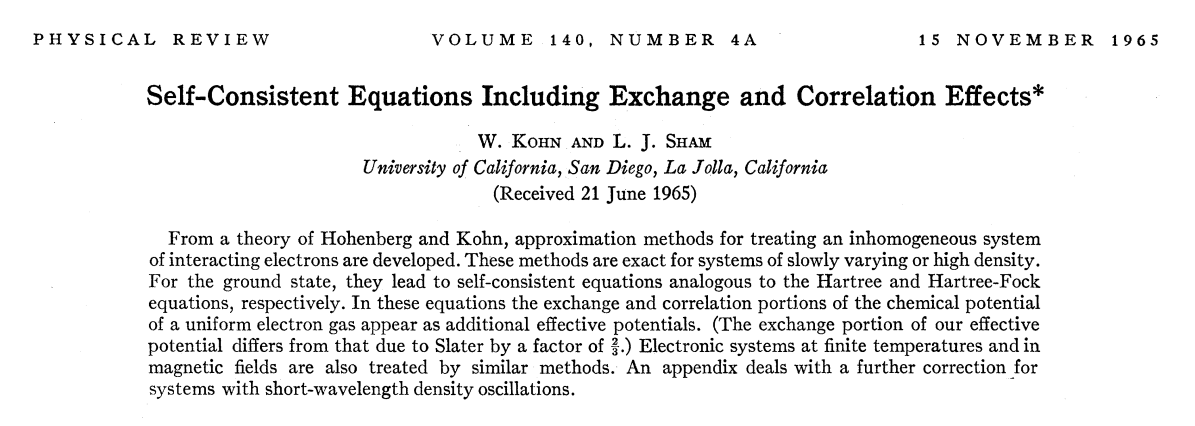
\includegraphics[width=\linewidth]{fig/kohn_sham_abstract.png}}
    \caption{บทคัดย่อของบทความงานวิจัยที่นำเสนอทฤษฎีบท Kohn-Sham ในปี ค.ศ. 1965}
    \label{fig:kohn_sham_abs}
\end{figure}

สำหรับการแก้ปัญหาดังกล่าวนั้น ในปี ค.ศ. 1965 ศาสตราจารย์ Walter Kohn และศาสตราจารย์ Lu Jeu Sham (University of California, San Diego) ก็ได้นำเสนอบทความงานวิจัย (หนึ่งปีหลังจากนำเสนอทฤษฎี Pure (Orbital-free) DFT) โดยได้เสนอการคำนวณฟังก์ชันของพลังงานโดยใช้ระบบที่อิเล็กตรอนไม่มีอันตรกิริยาต่อกัน (Non-interacting Electrons) แทนการแก้ผ่านระบบที่อิเล็กตรอนมีอันตรกิริยาต่อกัน\autocite{kohn1965} ซึ่งมีข้อดีคือทำให้ DFT มีความแม่นยำมากขึ้นเพราะว่าพลังงานจลน์ของระบบที่อิเล็กตรอนแต่ละตัวไม่ขึ้นหรือมีความสัมพันธ์กับอิเล็กตรอนตัวอื่น ๆ นั้นมีสมการที่เรารู้หน้าตาแน่นอน จึงไม่มีความจำเป็นที่จะต้องประมาณค่าฟังก์ชันนอลของพลังงานจลน์ในรูปของความหนาแน่นอีกต่อไป โดยในเวลาต่อมาทฤษฎีนี้คือ Kohn-Sham DFT นั่นเอง
\idxen{Density Functional Theory!Kohn-Sham Theorem}

%--------------------------
\subsection{จาก Hohenberg-Kohn สู่ Kohn-Sham}
\label{ssec:from_hk_to_ks}
%--------------------------

ในหัวข้อนี้เราจะมารู้จักกับความแตกต่างระหว่างระบบที่อิเล็กตรอนมีอันตรกิริยาต่อกัน (Interacting Electrons) และไม่มีอันตรกิริยาต่อกัน (Non-interacting Electrons) กันให้มากขึ้น เพราะว่าเป็นระบบที่ถูกนำมาใช้ในการพิจารณาความหนาแน่นของโมเลกุล

ตามที่ Kohn กับ Sham ได้เสนอการแก้ปัญหาของ Pure DFT โดยการเปลี่ยนมาพิจารณาระบบที่อิเล็กตรอนไม่มีอันตรกิริยาต่อกันแทนนั้น จริง ๆ แล้ว Wavefunction และความหนาแน่นของทั้งสองระบบนั้นแตกต่างกันอย่างสิ้นเชิง แต่ว่าทริคของวิธี Kohn-Sham นั้นคือทำการจำลองหรือสร้างระบบอิเล็กตรอนที่ไม่มีอันตรกิริยาต่อกันแบบปลอม ๆ ขึ้นมา (Fictitious Non-interacting Electron System) หรืออาจจะเรียกว่าระบบอิเล็กตรอนแบบเสริมก็ได้ (Auxiliary Non-interacting Electron System)\autocite{martin2020} โดยบังคับให้ความหนาแน่นของระบบนี้มีค่าเท่ากันกับความหนาแน่นของระบบที่อิเล็กตรอนมีอันตรกิริยาต่อกัน ดังนั้นความท้าทายจึงเปลี่ยนจากการหาฟังก์ชันนอลสากลสำหรับ Pure DFT มาเป็นการหาระบบที่อิเล็กตรอนไม่มีอันตรกิริยากันแบบปลอม ๆ ที่มีความหนาแน่นเท่ากัน ซึ่งการใช้ทริคนี้ทำให้เราไม่ต้องมาประมาณค่าพลังงานจลน์และทำให้การคำนวณ DFT นั้นมีความแม่นยำมากขึ้นเพราะว่าเรามีผลเฉลยที่แน่นอนของพลังงานตามที่ได้อธิบายไว้ก่อนหน้านี้ในย่อหน้าสุดท้ายของหัวข้อที่ \ref{ssec:univer_functional}
\idxboth{ระบบอิเล็กตรอน}{Electron System}
\idxboth{ระบบอิเล็กตรอนที่ไม่มีอันตรกิริยาต่อกัน}{Non-interacting Electron System}
\idxboth{ระบบอิเล็กตรอน!แบบเสริม}{Auxiliary}

\begin{figure}[H]
    \centering
    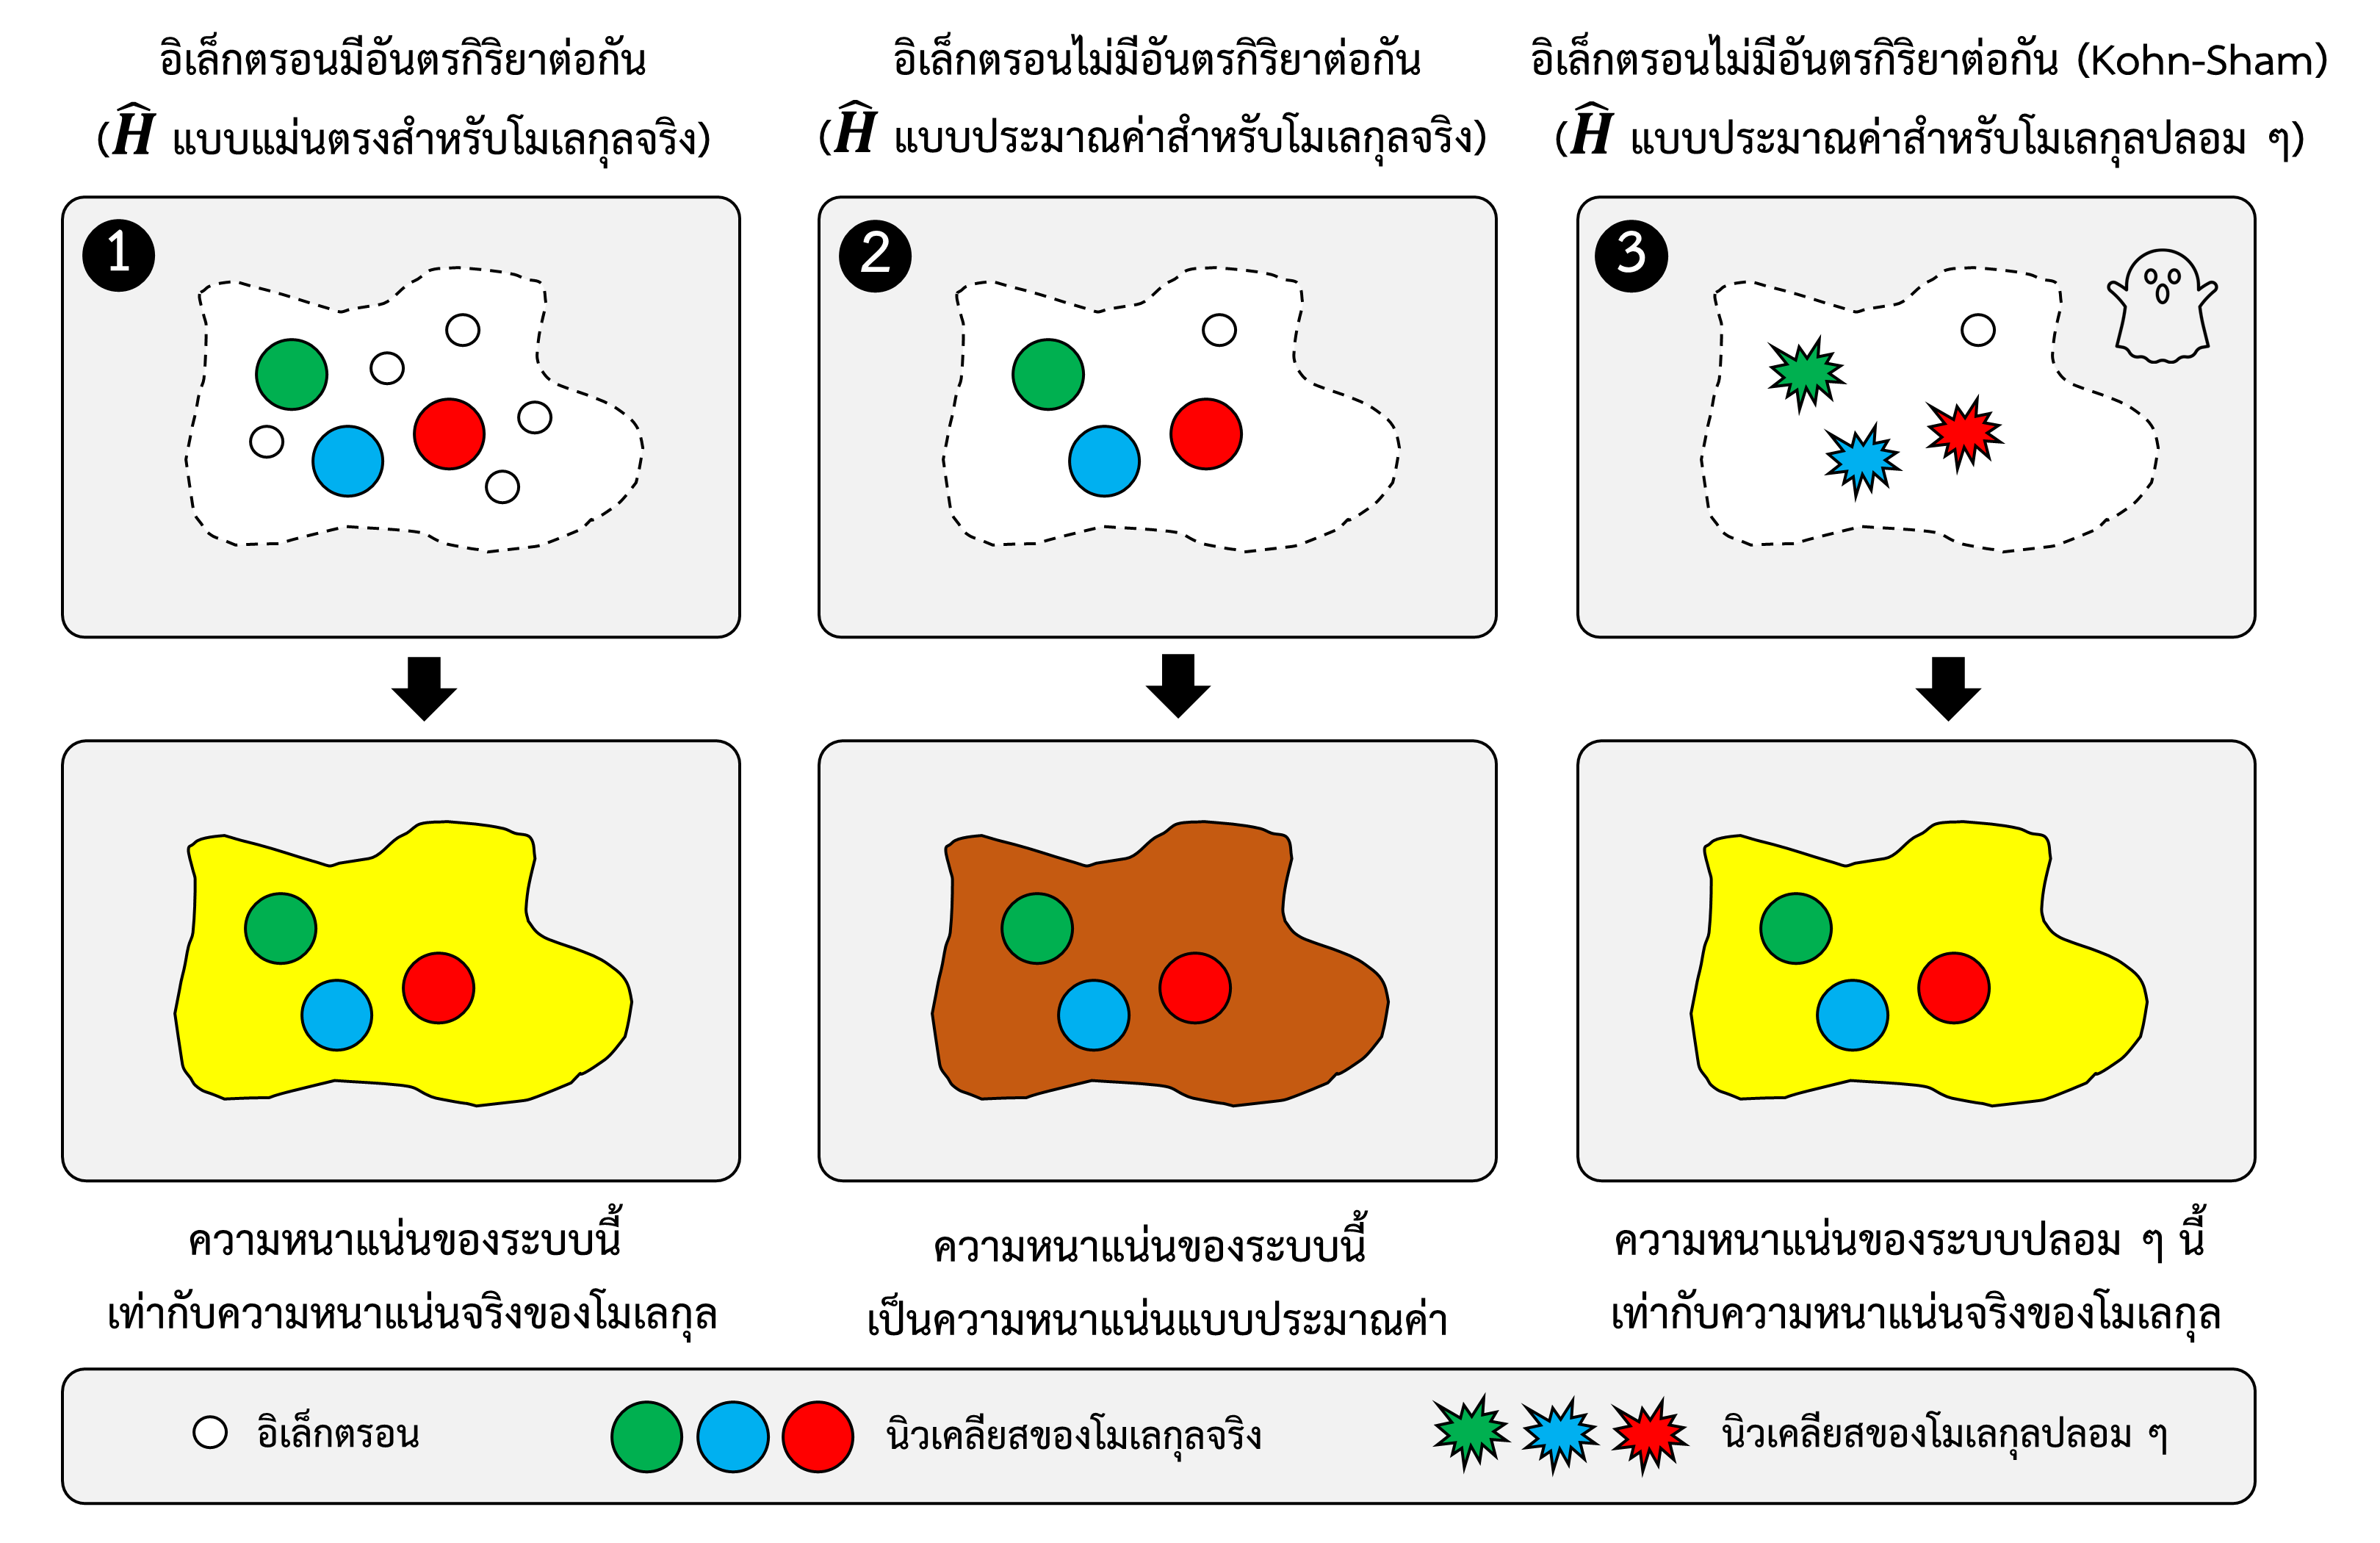
\includegraphics[width=\linewidth]{fig/electron_system.png}
    \caption{การเปรียบเทียบแบบจำลองของ (1) ระบบที่อิเล็กตรอนมีอันตรกิริยาต่อกัน, (2) ระบบที่อิเล็กตรอนไม่มีอันตรกิริยาต่อกัน, และ (3) ระบบที่อิเล็กตรอนไม่มีอันตรกิริยาต่อกันของโมเลกุลปลอมตามทฤษฎี Kohn-Sham}
    \label{fig:electron_system}
\end{figure}

เพื่อให้ผู้อ่านเข้าใจได้ง่ายขึ้นว่าทำไมระบบที่อิเล็กตรอนไม่มีอันตรกิริยาต่อกันของ Kohn-Sham นั้นถึงมีความหนาแน่นเท่ากันกับระบบที่อิเล็กตรอนมีอันตรกิริยาต่อกัน ให้ผู้อ่านเริ่มด้วยการศึกษาภาพที่ \ref{fig:electron_system} ซึ่งเป็นการเปรียบเทียบระหว่างโมเดลของอิเล็กตรอนที่แตกต่างกัน

\begin{itemize}[topsep=0pt,noitemsep]\setlength\itemsep{0.5em}
    \item ระบบที่ 1 คือระบบที่อิเล็กตรอนมีอันตรกิริยาต่อกัน ซึ่งเราสามารถหาผลเฉลยแบบแม่นตรงของ Wavefunction ของระบบนี้ได้ และความหนาแน่นของโมเดลนี้จะเท่ากับความหนาแน่นของโมเลกุลจริงด้วย

    \item ระบบที่ 2 ระบบที่อิเล็กตรอนไม่มีอันตรกิริยาต่อกัน หมายความว่าอิเล็กตรอนแต่ละตัวจะมี Hamiltonian Operator เป็นของตัวเอง ซึ่งอิเล็กตรอนแต่ละตัวจะวิ่งอยู่ภายในสนามของศักย์เฉลี่ย (Average Potential) ที่เกิดจากอิเล็กตรอนตัวอื่นในระบบ สำหรับระบบนี้เราจะทำการรวม Hamiltonian ของอิเล็กตรอนแต่ละตัวเข้าด้วยกันเพื่อประมาณค่า Wavefunction สำหรับอิเล็กตรอนทุกตัว

    \item ระบบที่ 3 จะคล้ายกับระบบที่ 2 แต่จะมีความแตกต่างกันที่ศักย์เฉลี่ยที่กระทำต่ออิเล็กตรอน กล่าวคือในระบบนี้ (เรียกว่าระบบอิเล็กตรอนของ Kohn-Sham ก็ได้) ศักย์เฉลี่ยที่เกิดขึ้นจะมาจากระบบของอิเล็กตรอนแบบปลอม ๆ (Fictitious System of Electrons) โดยเราจะทำการรวม Wavefunction ของอิเล็กตรอน (Molecular Orbitals) เข้าด้วยกันเพื่อประมาณค่า Wavefunction สำหรับอิเล็กตรอนทุกตัว ซึ่งความหนาแน่นของระบบ Kohn-Sham นี้จะมีค่าเท่ากับความหนาแน่นของระบบที่เป็นโมเลกุลจริง ๆ นั่นคือเท่ากับความหนาแน่นของระบบที่ 1 ด้วย
\end{itemize}

%--------------------------
\subsection{แฮมิลโทเนียนสำหรับอิเล็กตรอนที่ไม่มีอันตรกิริยาต่อกัน}
\label{ssec:hamil_noninter_elec}
%--------------------------

การที่เราเปลี่ยนมาพิจารณาระบบที่อิเล็กตรอนไม่มีอันตรกิริยาต่อกันแทนนั้น เราสามารถเปลี่ยนเทอมที่เป็นพลังงานที่เกิดจากการผลักกันของอิเล็กตรอน (Direct Interaction) ให้เป็นโอเปอเรเตอร์สำหรับอิเล็กตรอน 1 ตัวได้ (เพราะว่าอิเล็กตรอนทุกตัวเป็นอิสระและไม่ขึ้นต่อกันอีกต่อไปแล้ว) ซึ่งโอเปอเรเตอร์ที่ว่านั้นคือพลังงานศักย์ที่อธิบายค่าเฉลี่ยของผลที่เกิดจากอันตรกิริยาระหว่างอิเล็กตรอน (Average Effect) อธิบายง่าย ๆ คือเราใช้เทอมนี้เป็นตัวแทนของอันตรกิริยาระหว่างอิเล็กตรอนในระบบที่อิเล็กตรอนไม่มีอันตรกิริยาต่อกัน (เป็นเทอมที่เป็นส่วนเติมเต็ม) โดยเราสามารถพิสูจน์แฮมิลโทเนียน (Hamiltonian) ของ Effective Interaction สำหรับอิเล็กตรอนที่ไม่มีอันตรกิริยาได้จาก Hamiltonian แบบดั้งเดิม ดังต่อไปนี้
\idxen{Density Functional Theory!Effective Interaction}
\idxboth{แฮมิลโทเนียน}{Hamiltonian}

\begin{align}\label{eq:hamil_inter_elec}
    \hat{H}_{\text{el}} & = \sum^{N_{\text{el}}}_{i=1} -\frac{1}{2} \nabla^{2}_{i}
    + \sum^{N_{\text{el}}}_{i=1} \sum^{N_{\text{el}}}_{j=i+1} \frac{1}{|\bm{r}_{i}-\bm{r}_{j}|}
    + \sum^{N_{\text{el}}}_{i=1} V_{\text{ext}}(\bm{r}_{i})
\end{align}

\noindent สมการที่ \eqref{eq:hamil_inter_elec} นี้จะเปลี่ยนเป็นสมการของ Hamiltonian สำหรับ Effective Interaction ได้ดังนี้

\begin{align}\label{eq:hamil_noninter_eff_full}
    \hat{H}_{\text{eff}} & = \sum^{N_{\text{el}}}_{i=1} -\frac{1}{2} \nabla^{2}_{i}
    + \sum^{N_{\text{el}}}_{i=1} V_{\text{aver}}(\bm{r}_{i})
    + \sum^{N_{\text{el}}}_{i=1} V_{\text{ext}}(\bm{r}_{i}) \nonumber                                                            \\
                         & = \sum^{N_{\text{el}}}_{i=1} -\frac{1}{2} \nabla^{2}_{i}
    + \sum^{N_{\text{el}}}_{i=1} \{ V_{\text{aver}}(\bm{r}_{i}) + V_{\text{ext}}(\bm{r}_{i}) \} \nonumber                        \\
                         & = \sum^{N_{\text{el}}}_{i=1} -\frac{1}{2} \nabla^{2}_{i}
    + \sum^{N_{\text{el}}}_{i=1} V_{\text{eff}}(\bm{r}_{i}) \nonumber                                                            \\
                         & = \sum^{N_{\text{el}}}_{i=1} \{ -\frac{1}{2} \nabla^{2}_{i} + V_{\text{eff}}(\bm{r}_{i}) \} \nonumber \\
                         & = \sum^{N_{\text{el}}}_{i=1} \hat{h}(\bm{r}_{i})
\end{align}

จากการพิสูจน์ข้างต้นจะได้ว่าสุดท้ายแล้ว Hamiltonian ทั้งหมดของระบบที่อิเล็กตรอนไม่มีอันตรกิริยาต่อกันนั้นคือผลรวมของ Hamiltonian ของอิเล็กตรอนหนึ่งตัว (1 Hamiltonian ต่ออิเล็กตรอน 1 ตัว) กล่าวคือจากการพิสูจน์ของสมการที่ \eqref{eq:hamil_noninter_eff_full} เราจะได้ความสัมพันธ์ที่สั้นและกระชับ ดังนี้

\begin{equation}\label{eq:hamil_noninter_eff}
    \hat{H}_{\text{eff}} = \sum^{N_{\text{el}}}_{i=1} \hat{h}(\bm{r}_{i})
\end{equation}

นอกจากนี้เราสามารถเขียนและแก้ Schr\"{o}dinger Equation สำหรับ Hamiltonian ของอิเล็กตรอนแต่ละตัวแยกกันได้ดังนี้

\begin{equation}\label{eq:hamil_one_elec_mo}
    \hat{h}(\bm{r}_{i}) \underbrace{\psi_{a}(\bm{r}_{i})}_{\text{MOs}} =
    \underbrace{\epsilon_{a}}_{\text{Energy}} \psi_{a}(\bm{r}_{i})
\end{equation}

\noindent ซึ่งจากตรงนี้เราสามารถคำนวณหาออร์บิทัลเชิงโมเลกุล (Molecular Orbitals หรือ MOs) และพลังงานที่สอดคล้องกันได้

%--------------------------
\subsection{ออร์บิทัลเชิงโมเลกุลและผลคูณฮาร์ทรี}
\label{ssec:mol_orb_hartree_prod}
\idxboth{ออร์บิทัลเชิงโมเลกุล}{Molecular Orbital}
%--------------------------

เนื่องจากว่า Kohn-Sham DFT นั้นอ้างอิงอยู่กับออร์บิทัลเชิงโมเลกุล (Molecular Orbital หรือ MO) เราจึงควรที่จะเข้าใจเกี่ยวกับ MO ด้วย ซึ่ง MO นั้นจริง ๆ แล้วคือฟังก์ชันคลื่นของอิเล็กตรอนหนึ่งตัว (One-electron Wavefunction) โดย MO ที่ประกอบไปด้วยพิกัดเชิงพื้นที่ (Spatial Coordinates) และพิกัดเชิงสปิน (Spin Coordinates) นั้นจะมีชื่อเรียกว่าออร์บิทัลเชิงสปิน (Spin Orbital) ซึ่งเป็นผลคูณของทั้ง Spatial Function และ Spin Function ตามสมการดังต่อไปนี้
\idxboth{ออร์บิทัลเชิงโมเลกุล}{Molecular Orbital}
\idxboth{พิกัดเชิงพื้นที่}{Spatial Coordinates}
\idxboth{พิกัดเชิงสปิน}{Spin Coordinates}
\idxboth{ออร์บิทัลเชิงสปิน}{Spin Orbital}

\noindent สปินขึ้น (Up Spin):

\begin{equation}\label{eq:hamil_spin_orb_up}
    \underbrace{\chi^{\uparrow}(\bm{x})}_{\text{Spin Orbital}} =
    \underbrace{\psi(\bm{r})}_{\text{Spatial}} \underbrace{\alpha(\omega)}_{\text{Spin}}
\end{equation}

\noindent สปินลง (Down Spin)

\begin{equation}\label{eq:hamil_spin_orb_down}
    \underbrace{\chi^{\downarrow}(\bm{x})}_{\text{Spin Orbital}} =
    \underbrace{\psi(\bm{r})}_{\text{Spatial}} \underbrace{\beta(\omega)}_{\text{Spin}}
\end{equation}

\noindent ถึงแม้ว่า Hamilnotian สำหรับอิเล็กตรอนหนึ่งตัว (สมการที่ \eqref{eq:hamil_one_elec_mo}) เป็นฟังก์ชันที่ขึ้นอยู่กับเพียงแค่ Spatial Coordinates เท่านั้น เราก็สามารถใช้ Spin Orbitals ซึ่งก็เป็น Eigenfunction ได้เช่นกัน ดังนั้นจากสมการที่ \eqref{eq:hamil_one_elec_mo} เราจะได้ Schr\"{o}dinger Equation ที่ใช้ Spin Orbitals สำหรับอิเล็กตรอนตัวที่ $i$ ดังนี้

\begin{equation}\label{eq:hamil_spin_orb}
    \hat{h}(\bm{r}_{i}) \underbrace{\chi_{a}(\bm{r}_{i})}_{\text{MOs}} =
    \underbrace{\epsilon_{a}}_{\text{Energy}} \chi_{a}(\bm{r}_{i})
\end{equation}

คราวนี้มาดูตัวอย่างง่าย ๆ นั่นคือระบบที่มีอิเล็กตรอนสองตัวที่ไม่มีอัตรกิริยาต่อกัน (Two Non-interacting Electrons) โดยเราสามารถเขียน Wavefunction สำหรับทั้งสองอิเล็กตรอนได้ดังนี้

\begin{align}\label{eq:hamil_spin_orb_two_elec}
    \hat{h}(\bm{r}_{1}) \underbrace{\chi_{a}(\bm{r}_{1})}_{\text{MOs}} & =
    \underbrace{\epsilon_{a}}_{\text{Energy}} \chi_{a}(\bm{r}_{1})         \\
    \hat{h}(\bm{r}_{2}) \underbrace{\chi_{a}(\bm{r}_{2})}_{\text{MOs}} & =
    \underbrace{\epsilon_{a}}_{\text{Energy}} \chi_{a}(\bm{r}_{2})
\end{align}

ถ้าเป็นกรณีหลายวัตถุ (Many-body) แบบที่มีอิเล็กตรอน $N_{\text{el}}$ ตัวในระบบที่อิเล็กตรอนไม่มีอัตรกิริยาต่อกัน เราสามารถเขียนผลเฉลยแบบแม่นตรง (Exact Solution) ของ Schr\"{o}dinger Equation ได้ดังนี้

\begin{multline}\label{eq:schro_eq_spin_orb_n_elec}
    \left [ \sum_{i=1}^{N_{\text{el}}} \hat{h}(\bm{r}_{i}) \right ] \chi_{a}(\bm{x}_{1}) \chi_{b}(\bm{x}_{2})
    \cdots \chi_{z}(\bm{x}_{N_{el}}) = \\
    (\epsilon_{a} + \epsilon_{b} \dots \epsilon_{z}) \chi_{a}(\bm{x}_{1}) \chi_{b}(\bm{x}_{2}) \cdots
    \chi_{z}(\bm{x}_{N_{\text{el}}})
\end{multline}

\noindent ซึ่งเราสรุปได้ว่า \textbf{\textit{พลังงานรวม (Eigenvalue) ของระบบหรือโมเลกุลของเรานั้นจริง ๆ แล้วมีค่าเท่ากับผลรวมของพลังงานของ Spin Orbital ของอิเล็กตรอนแต่ละตัวรวมกัน}}

ประเด็นต่อมาก็คือตามสมการที่ \eqref{eq:schro_eq_spin_orb_n_elec} นั้น เราสามารถเขียนผลคูณของ Spin Orbitals แต่ละตัวให้เป็น Wavefunction ของระบบที่อิเล็กตรอนเป็นอิสระต่อกันได้ ดังนี้

\begin{equation}\label{eq:hartree_product}
    \Psi_{\text{eff}} = \chi_{a}(\bm{x}_{1}) \chi_{b}(\bm{x}_{2}) \cdots \chi_{z}(\bm{x}_{N_{\text{el}}})
\end{equation}

\noindent โดยเราเรียก Wavefunction ในสมการที่ \eqref{eq:hartree_product} นี้ว่า \enquote{ผลคูณฮาร์ทรี (Hartree Product)} ซึ่งการเขียน Wavefunction แบบนี้ถูกต้องตามหลักคณิตศาสตร์ทุกประการ แต่ทว่าตามหลักกลศาสตร์ควอนตัม Hartree Product นั้นขัดแย้งกับคุณสมบัติข้อหนึ่งของ Wavefunction นั่นก็คือ Wavefunction จะต้องมีปฏิสมมาตร (Antisymmetry) กล่าวคือถ้าเรามีการสลับตำแหน่งของ Spatial Coordinate หนึ่งครั้ง เครื่องหมายของ Wavefunction ก็จะเปลี่ยนไป (จากลบเป็นบวกหรือจากบวกเป็นลบ) แต่ว่าในกรณีของ Hartree Product นั้นเนื่องจากว่าอิเล็กตรอนทุกตัวเป็นอิสระต่อกัน จึงทำให้ Wavefunction ที่เป็นผลคูณระหว่าง Spin Orbitals นั้นไม่มีคุณสมบัติ Antisymmetry ดังนั้นเป้าหมายต่อไปของเราก็คือการหารูปแบบ (Form) ทางคณิตศาสตร์แบบอื่นที่สามารถอธิบาย Wavefunction และมีคุณสมบัติของ Antisymmetry อยู่ด้วย
\idxboth{ผลคูณฮาร์ทรี}{Hartree Product}
\idxboth{ปฏิสมมาตร}{Antisymmetry}

%--------------------------
\subsection{จากผลคูณฮาร์ทรีสู่ดีเทอร์มิแนนต์ของสเลเตอร์}
\label{ssec:hartree_prod_to_slater_deter}
\idxboth{ออร์บิทัลเชิงโมเลกุล}{Molecular Orbital}
%--------------------------

เมื่อผลคูณฮาร์ทรี (Hartree Product) ไม่เหมาะสมที่จะถูกนำมาใช้ในการสร้าง Wavefunction ดังนั้นจึงได้มีการพัฒนาสิ่งที่เรียกว่าดีเทอร์มิแนนต์ของสเลเตอร์ (Slater Determinant) ขึ้นมา โดยตั้งชื่อตามนามสกุลของศาสตราจารย์ John C. Slater นักฟิสิกส์ชาวอเมริกา ซึ่งแนวคิดของ Slater Determinant นั้นก็คือการใช้ผลรวมเชิงเส้น (Linear Combination) ของ Hartree Product นั่นเอง\autocite{slater1929} ตัวอย่างเช่นกรณีที่ระบบมีอิเล็กตรอนสองตัว เราจะได้ว่า Wavefunction ที่เขียนในรูปของผลรวมเชิงเส้นของ Hartree Product ที่มีคุณสมบัติ Antisymmetry มีดังนี้

\begin{equation}\label{eq:lin_com_hartree_prod}
    \Psi(\bm{x}_{1}, \bm{x}_{2}) = \chi_{1}(\bm{x}_{1})\chi_{2}(\bm{x}_{2}) -
    \chi_{2}(\bm{x}_{1})\chi_{1}(\bm{x}_{2})
\end{equation}

\noindent ซึ่งสามารถเขียนเป็นดีเทอร์มีแนนต์ (Determinant) ของเมทริกซ์ออร์บิทัลเชิงสปินได้ดังนี้

\begin{align}\label{eq:slater_det_2e}
    \Psi(\bm{x}_{1}, \bm{x}_{2}) & =
    \det \begin{pmatrix}
             \chi_{1}(\bm{x}_{1}) & \chi_{2}(\bm{x}_{1}) \\
             \chi_{1}(\bm{x}_{2}) & \chi_{2}(\bm{x}_{2})
         \end{pmatrix} \nonumber                             \\
                                 & = \begin{vmatrix}
                                         \chi_{1}(\bm{x}_{1}) & \chi_{2}(\bm{x}_{1}) \\
                                         \chi_{1}(\bm{x}_{2}) & \chi_{2}(\bm{x}_{2})
                                     \end{vmatrix}
\end{align}

\noindent โดยเราเรียกสมการที่ \eqref{eq:slater_det_2e} ที่เป็น Wavefunction นี้ว่า Slater Determinant ซึ่งสามารถที่จะทำให้มีรูปแบบทั่วไป (Generalized) สำหรับระบบที่มีอิเล็กตรอนกี่ตัวก็ได้ ($N$-electron System) นอกจากนี้ ตามที่ได้อธิบายไว้ก่อนหน้านี้ว่า Slater Determinant นั้นมีคุณสมบัติ Antisymmetry ซึ่งทำให้ Wavefunction นั้นจะมีการเปลี่ยนเครื่องหมายทุกครั้งที่เราทำการสลับแถวหรือสลับหลัก

สำหรับ Slater Determinant ของระบบที่มี $N$ อิเล็กตรอนนั้นเราสามารถกำหนดได้ดังนี้\autocite{szabo1996}

\begin{equation}\label{eq:slater_det_N_elec}
    \Psi(\bm{x}_{1}, \bm{x}_{2}, \dots, \bm{x}_{N}) =
    \frac{1}{\sqrt{N!}}
    \begin{vmatrix}
        \chi_{1}(\bm{x}_{1}) & \chi_{2}(\bm{x}_{1}) & \cdots & \chi_{N}(\bm{x}_{1}) \\
        \chi_{1}(\bm{x}_{2}) & \chi_{2}(\bm{x}_{2}) & \cdots & \chi_{N}(\bm{x}_{2}) \\
        \vdots               & \vdots               &        & \vdots               \\
        \chi_{1}(\bm{x}_{N}) & \chi_{2}(\bm{x}_{N}) & \cdots & \chi_{N}(\bm{x}_{N})
    \end{vmatrix}
\end{equation}

\noindent โดยที่ $1/\sqrt{N!}$ คือค่าคงที่ของการทำ Normalization นอกจากนี้เรายังสามารถเขียนสมการที่ \eqref{eq:slater_det_N_elec} ให้สั้นลงได้โดยใช้สัญกรณ์เค็ท (Ket Notation) ดังนี้

\begin{equation}\label{eq:slater_det_ket}
    \Psi(\bm{x}_{1}, \bm{x}_{2}, \cdots, \bm{x}_{N}) =
    \ket{\chi_{1}(\bm{x}_{N}) \chi_{2}(\bm{x}_{N}) \cdots \chi_{N}(\bm{x}_{N})}
\end{equation}

\noindent หรือจะเขียนให้สั้นและกระชับกว่านี้ก็ได้ ดังนี้

\begin{equation}\label{eq:slater_det_ket_short}
    \Psi(\bm{x}_{1}, \bm{x}_{2}, \dots, \bm{x}_{N}) =
    \ket{1, 2, \cdots, N}
\end{equation}

คุณสมบัติอีกอย่างหนึ่งที่ Slater Determinant มีนั่นก็คือประพฤติตัวตามหลักของเพาลี (Pauli Principle) นั่นคือ Spatial Orbital นั้นจะมีอิเล็กตรอนได้สูงสุดไม่เกิน 2 ตัว และอิเล็กตรอนทั้งสองตัวนั้นจะต้องมีสปินที่ตรงข้ามกัน\autocite{atkins2010}
\idxboth{หลักของเพาลี}{Pauli Principle}

ณ จุด ๆ นี้เมื่อเราสามารถใช้ Slater Determinant เป็น Wavefunction ได้แล้ว เราก็สามารถหาความหนาแน่นของอิเล็กตรอนได้เช่นกัน โดยสำหรับระบบที่มีจำนวนอิเล็กตรอนเป็นเลขคู่ (Closed-shell) และอิเล็กตรอนทุกตัวถูกบรรจุอยู่ใน Spatial Orbitals จะได้ว่า

\begin{equation}\label{eq:density_slater}
    n(\bm{r}) = 2 \sum_{i=1}^{N_{el}/2} |\psi_{i}(\bm{r})|^{2}
\end{equation}

ดังนั้นเราจึงสรุปได้ว่า  \textbf{\textit{ความหนาแน่นของอิเล็กตรอนของฟังก์ชันคลื่นแบบ Slater Determinant นั้นมีค่าเท่ากับผลรวมของยกกำลังสองของออร์บิทัลที่บรรจุอิเล็กตรอน (Occupied Orbital)}}

%--------------------------
\subsection{Orbital-free DFT ปะทะ Kohn-Sham DFT}
\label{ssec:orb_free_vs_kohn_sham_dft}
\idxen{Density Functional Theory!Orbital-free}
\idxen{Density Functional Theory!Kohn-Sham}
%--------------------------

\begin{figure}[H]
    \centering
    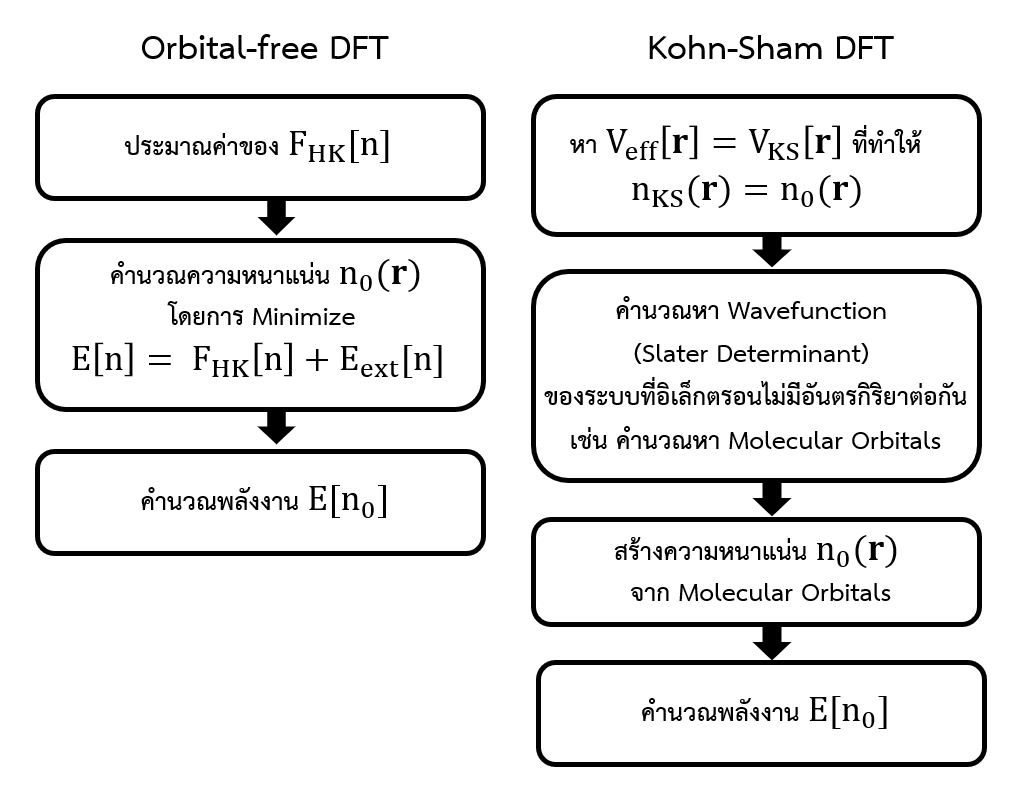
\includegraphics[width=0.9\linewidth]{fig/orb_free_vs_kohn_sham.png}
    \caption{การเปรียบเทียบขั้นตอนการคำนวณพลังงานของระบบด้วยวิธี Orbital-free DFT และวิธี Kohn-Sham DFT}
    \label{fig:orb_free_vs_kohn_sham}
\end{figure}

ภาพที่ \ref{fig:orb_free_vs_kohn_sham} แสดงการเปรียบเทียบขั้นตอนการคำนวณพลังงานของระบบที่อิเล็กตรอนไม่มีอันตรกิริยาต่อกันด้วยวิธี Orbital-free DFT ซึ่งเป็นการคำนวณผ่าน Universal Function ของ Hohenberg-Kohn และวิธี Kohn-Sham DFT ซึ่งเป็นการคำนวณผ่านความหนาแน่นซึ่งอ้างอิงกับ Molecular Orbitals ผู้อ่านสามารถศึกษาโค้ดของ Kohn-Sham DFT และการเขียนนำฟังก์ชันนอลจาก LibXC มาใช้เพื่อคำนวณพลังงานได้ที่ซอร์สโค้ดของโปรแกรม PySCF (\url{https://github.com/pyscf/pyscf/tree/master/pyscf/dft}) ตัวอย่างเช่น โค้ดของฟังก์ชัน \pyinline{get_veff} บรรทัดที่ 30-105 (\url{https://github.com/pyscf/pyscf/blob/master/pyscf/dft/uks.py#L30-L105}) สำหรับ Unrestricted Kohn-Sham ซึ่งเป็นฟังก์ชันที่คำนวณผลรวมของพลังงานศักย์คูลอมป์ (Coulomb Energy) และพลังงานแลกเปลี่ยน-สหสัมพันธ์ (Exchange-Correlation Energy)

จากที่ได้อธิบายมาตั้งแต่ต้นเราสามารถสรุปเปรียบเทียบฟังก์ชันของพลังงานที่คำนวณด้วยวิธี Orbital-free DFT และวิธี Kohn-Sham DFT ได้ดังนี้

\noindent $\bullet$ \textbf{Orbital-free DFT}

\begin{equation}\label{eq:ener_orb_free}
    E[n] = E_{\text{kin}}[n] + E_{\text{Coul}}[n] + E_{\text{XC}}[n] + E_{\text{Ext}}[n]
\end{equation}

\noindent อุปสรรคในการใช้สมการที่ \eqref{eq:ener_orb_free} ก็คือเราไม่มีผลเฉลยที่ถูกต้องของฟังก์ชันนอลของพลังงานจลน์

\noindent $\bullet$ \textbf{Kohn-Sham DFT}

\begin{multline}\label{eq:ener_kohn_sham}
    E[n] = E_{\text{kin,KS}}[n] + (E_{\text{kin}}[n] - E_{\text{kin,KS}}[n]) + E_{\text{Coul}}[n] \\
    + E_{\text{XC}}[n] + E_{\text{Ext}}[n]
\end{multline}

\noindent โดยที่ $E_{\text{kin,KS}}[n]$ คือพลังงานของระบบที่อิเล็กตรอนไม่มีอันตรกิริยาต่อกัน (ระบบอิเล็กตรอนของ Kohn-Sham) ซึ่งเรารู้ผลเฉลยแบบแม่นตรงของ $E_{\text{kin,KS}}[n]$ ถึงแม้ว่าจะอยู่ในเทอมของ Molecular Orbitals และไม่ใช่ความหนาแน่นก็ตาม นอกจากนี้เทอมที่น่าสนใจอีกเทอมหนึ่งก็คือความแตกต่างระหว่างพลังงานจลน์จริง ๆ ของระบบกับพลังงานจลน์ของ Kohn-Sham $(E_{\text{kin}}[n] - E_{\text{kin,KS}}[n])$ นั้นมีค่าน้อยกว่าความคลาดเคลื่อนในประมาณค่าของ $E_{\text{kin,KS}}[n]$ ของ Orbital-free DFT มาก ดังนั้น Kohn-Sham DFT จึงสามารถคำนวณพลังงานเชิงอิเล็กทรอนิกส์ได้แม่นยำมากกว่าวิธี Orbital-free DFT

%--------------------------
\subsection{พลังงานของ Kohn-Sham}
\label{ssec:kohn_sham_ener_expr}
\idxth{ทฤษฎีฟังก์ชันนอลความหนาแน่น!พลังงาน Kohn-Sham}
\idxen{Density Functional Theory!Kohn-Sham Energy}
%--------------------------

เพื่อไม่ให้ผู้อ่านสับสนเราสามารถสรุปสมการที่ใช้ในการคำนวณพลังงานของระบบอิเล็กตรอนของ Kohn-Sham ดังนี้

\begin{framed}
    ฟังก์ชันนอลของพลังงานรวม $=$ พลังงานจลน์ที่เป็นฟังก์ชันนอลของ MOs $+$ พลังงานเทอมอื่น ๆ ที่เหลือที่เป็นฟังก์ชันนอลของความหนาแน่น
\end{framed}

\noindent ซึ่งเขียนได้เป็นสมการดังนี้

\begin{align}
    \label{eq:kohn_sham_ener_1}
    E_{\text{KS}}[n] & = E_{\text{kin,KS}}[n] + E_{\text{Coul}}[n] + E_{\text{Ext}}[n] +
    \underbrace{E_{\text{XC}}[n] + (E_{\text{kin}}[n] - E_{\text{kin,KS}}[n])}_{\text{นำมารวมกันได้}}                           \\
    \label{eq:kohn_sham_ener_2}
                     & = 2 \sum^{N_{\text{el}}/2}_{i=1} \int \psi^{\ast}_{i}(\bm{r}) \left ( -\frac{1}{2}\nabla^{2} \right )
    + E_{\text{Coul}}[n] + E_{\text{Ext}}[n] + {E'}_{\text{XC}}[n]
\end{align}

\noindent นั่นคือความหนาแน่นของระบบที่อิเล็กตรอนที่มีอันตรกิริยาต่อกันถูกสร้างขึ้นจากออร๊บิทัลเชิงโมเลกุลของระบบที่อิเล็กตรอนไม่มีอันตรกิริยาต่อกันของ Kohn-Sham (Kohn-Sham MOs) ดังนั้นท้ายที่สุดแล้วเราสามารถสรุปได้อีกว่า \enquote{\textit{พลังงานของระบบของ Kohn-Sham นั้นเป็นฟังก์ชันนอลของ Kohn-Sham MOs นั่นเอง}}

ประเด็นก็คือเราจะต้องทำการประมาณค่าของเทอม ${E'}_{\text{XC}}[n]$ ซึ่งถึงแม้ว่าเทอมนี้จะมีการรวม Contribution จากพลังงานจลน์ของระบบเข้ามาด้วย (จากสมการที่ \eqref{eq:kohn_sham_ener_1} มาเป็นสมการที่ \eqref{eq:kohn_sham_ener_2}) แต่เราก็ยังเรียกเทอมนี้ว่า Exchange-Correlation Functional อยู่ครับ ซึ่งการหาเทอมนี้เป็นหนึ่งในหัวข้องานวิจัยที่สำคัญและมีกลุ่มวิจัยหลายกลุ่มให้ความสนใจเป็นอย่างมาก

%--------------------------
\subsection{การปรับหาค่าพลังงานให้ต่ำที่สุด}
\label{ssec:kohn_sham_ener_minimize}
\idxth{ทฤษฎีฟังก์ชันนอลความหนาแน่น!การปรับลดค่าพลังงาน Kohn-Sham}
\idxen{Density Functional Theory!Kohn-Sham Energy Minimization}
%--------------------------

เมื่อเรารู้แล้วว่าพลังงานรวมของระบบที่ถูกคำนวณด้วย Kohn-Sham DFT นั้นเป็นฟังก์ชันนอลของ MOs ของระบบที่อิเล็กตรอนไม่มีอันตรกิริยาต่อกันของ คำถามต่อมาที่เราจะต้องมาหาคำตอบก็คือเราจะคำนวณ Kohn-Sham MOs ได้อย่างไร ในหัวข้อก่อนหน้านี้ผู้อ่านได้ศึกษาไปแล้วว่าในการปรับลดค่าของพลังงานนั้นสามารถทำได้โดยการใช้หลักการแปรค่า (Variation Principle) ซึ่งจะเป็นการปรับลดค่าพลังงานรวมโดยเทียบกับความหนาแน่นเพื่อหาพลังงานของระบบ ณ สถานะพื้นโดยเราเรียกกระบวนการนี้ว่า Energy Minimization อย่างไรก็ตามเราไม่สามารถใช้เทคนิคนี้กับกรณีของ Kohn-Sham DFT ได้ เพราะว่าพลังงานรวมของ Kohn-Sham นั้นเป็นฟังก์ชันนอลของ MOs ดังนั้นเราจะต้องทำการ Minimize พลังงานโดยเทียบกับ MOs แทน ซึ่งความหนาแน่นของอิเล็กตรอนนั้นก็ขึ้นอยู่กับ MOs ด้วย

เนื่องจากว่าปัญหาการปรับลดค่าพลังงานรวมนั้นเป็นปัญหาค่าต่ำสุดที่มีหลายตัวแปรซึ่งเราสามารถใช้ตัวคูณลากรองจ์ (Langrange Multiplier) ได้ เริ่มต้นเรากำหนดชุดของ Langrange Multiplier แล้วทำการ Minimize ดังนี้

\begin{equation}\label{eq:langrange_mult}
    \Omega_{\text{KS}[n]} = E_{\text{KS}}[n] - 2 \sum^{N_{\text{el}}/2}_{i=1} \sum^{N_{\text{el}}/2}_{j=1}
    \epsilon_{ij} \left ( \int \phi^{\ast}_{i}(\bm{r}) \phi_{j}(\bm{r}) d\bm{r} - \delta_{ij} \right )
\end{equation}

\noindent ในการหาอนุพันธ์เชิงฟังก์ชันนอล (Functional Derivative) ของสมการที่ \eqref{eq:langrange_mult} เทียบกับออร์บิทัลเราสามารถใช้กฎลูกโซ่ได้ ดังนี้

\begin{equation}\label{eq:func_der_ener_chain_1}
    \fdv{\Omega_{\text{KS}[n]}}{\phi^{\ast}_{j}(\bm{r})} = \fdv{\Omega_{\text{KS}[n]}}{n(\bm{r})}
    \fdv{n(\bm{r})}{\phi^{\ast}_{j}(\bm{r})}
\end{equation}

\noindent เนื่องจากว่าเราทราบค่าของอนุพันธ์ของความหนาแน่นเทียบกับออร์บิทัล ดังต่อไปนี้

\begin{equation}\label{eq:func_der_den_chain}
    \fdv{n(\bm{r})}{\phi^{\ast}_{j}(\bm{r})} = 2 \phi^{\ast}_{j}(\bm{r})
\end{equation}

\noindent เมื่อเราแทนสมการ \eqref{eq:func_der_den_chain} เข้าไปในสมการที่ \eqref{eq:func_der_ener_chain_1} เราจะได้สมการคือ

\begin{equation}\label{eq:func_der_ener_chain_2}
    \fdv{\Omega_{\text{KS}[n]}}{\phi^{\ast}_{j}(\bm{r})} = \fdv{\Omega_{\text{KS}[n]}}{n(\bm{r})}
    \fdv{n(\bm{r})}{\phi^{\ast}_{j}(\bm{r})} = \fdv{\Omega_{\text{KS}[n]}}{n(\bm{r})} 2 \phi^{\ast}_{j}(\bm{r})
\end{equation}

\noindent นอกจากนี้เรามีเงื่อนไขเพิ่มเติมว่าอนุพันธ์เชิงฟังก์ชันนอลของพลังงานเมื่อเทียบกับออร์บิทัลนั้นจริง ๆ แล้วเท่ากับศูนย์ ดังนี้

\begin{equation}\label{eq:func_der_ener_chain_zero}
    \fdv{\Omega_{\text{KS}[n]}}{\phi^{\ast}_{j}(\bm{r})} = 0
\end{equation}

เมื่อรวมทุกอย่างเข้าด้วยกันเราจะพบว่าอนุพันธ์เชิงฟังก์ชันนอลของพลังงานนั้นสามารถเขียนกระจายได้เป็น

\begin{align}
    \fdv{\Omega_{\text{KS}[n]}}{\phi^{\ast}_{j}(\bm{r})}
     & = \begin{multlined}[t]
             2 \left ( -\frac{1}{2}\nabla^{2} \phi_{j}(\bm{r}) \right ) \\
             + 2 \left ( \fdv{E_{\text{Coul}}}{n} + \fdv{E_{\text{ext}}}{n} + \fdv{E_{\text{XC}}}{n} \right )
             \phi_{j}(\bm{r}) \\
             - 2 \sum^{N_{\text{el}}/2}_{i=1} \epsilon_{ij} \phi_{j}(\bm{r})
         \end{multlined} \\
     & = 0
\end{align}

เมื่อถึงขั้นตอนนี้แล้วขั้นตอนต่อไปก็คือเราสามารถทำการรวมออร์บิทัล $\{\phi\}$ ทั้งหมดเข้าด้วยกัน (โดยใช้ Summation สำหรับทุกดัชนี $i$) ให้เป็นออร์บิทัลใหม่โดยกำหนดด้วยตัวแปร $\{\psi\}$ ซึ่งเราจะได้สมการดังต่อไปนี้

\begin{equation}
    \left ( -\frac{1}{2}\nabla^{2} \psi_{j}(\bm{r}) \right )
    + \left ( \fdv{E_{\text{Coul}}}{n} + \fdv{E_{\text{ext}}}{n} + \fdv{E_{\text{XC}}}{n} \right )
    \psi_{j}(\bm{r}) - \epsilon_{j} \psi_{j}(\bm{r})
    = 0
\end{equation}

\noindent เมื่อทำการจัดรูปสมการโดยย้ายเทอมที่มีพลังงานของระบบมาทางด้านขวาของสมการแล้วทำการรวมเทอมฝั่งซ้ายซึ่งเป็นโอเปอเรเตอร์ดังนี้

\begin{align}
    \left \{ -\frac{1}{2}\nabla^{2} \left (
    + \fdv{E_{\text{Coul}}}{n} + \fdv{E_{\text{ext}}}{n} + \fdv{E_{\text{XC}}}{n} \right )
    \right \} \psi_{j}(\bm{r})
    = \epsilon_{j} \psi_{j}(\bm{r}) \nonumber \\
    \left ( -\frac{1}{2}\nabla^{2} + V_{\text{KS}}(\bm{r}) \right ) \psi_{j}(\bm{r})
    = \epsilon_{j} \psi_{j}(\bm{r}) \label{eq:func_der_ener_chain_full}
\end{align}

\noindent ซึ่งสมการที่ \eqref{eq:func_der_ener_chain_full} ก็คือ Schr\"{o}dinger Equation สำหรับหนึ่งอิเล็กตรอนนั่นเอง โดยเราสามารถแก้สมการเพื่อหา Kohn-Sham MOs ได้ อย่างไรก็ตาม เนื่องจากว่าเราไม่รู้ว่า MOs เริ่มต้นนั้นมีหน้าตาเป็นอย่างไร (Unknown) เราจึงไม่สามารถหาเฉลยแม่นตรงได้ ดังนั้นเราจึงจำเป็นต้องใช้วิธี Self-Consistent Field (SCF) ซึ่งเป็นวิธีวนซ้ำ (Iterative Method) โดนมีขั้นตอนคร่าว ๆ ดังต่อไปนี้

\begin{framed}
    \centering
    1. ทำการสร้างออร์บิทัลเชิงโมเลกุลเริ่มต้น (Initial Guess of MOs)
    \\ $\downarrow$ \\
    2. สร้าง Kohn-Sham Operator
    \\ $\downarrow$ \\
    3. คำนวณพลังงาน
    \\ $\downarrow$ \\
    4. เปรียบเทียบพลังงานของรอบปัจจุบันกับพลังงานของรอบที่แล้ว
    \\ $\downarrow$ \\
    5. ถ้าความแตกต่างของพลังงานและความหนาแน่น
    \\
    \vspace{0.5em}
    \begin{minipage}{0.6\linewidth}
        \begin{itemize}
            \item $>$ ค่า Cutoff $\rightarrow$ ขั้นตอนที่ 2
            \item $<$ ค่า Cutoff $\rightarrow$ สิ้นสุดการคำนวณ
        \end{itemize}
    \end{minipage}
\end{framed}

รายละเอียดของทฤษฎี DFT และการคำนวณด้วยคอมพิวเตอร์นั้นมีอีกเยอะมาก เช่น ฟังก์ชันพื้นฐาน (Basis Set) แต่ละประเภทและแต่ละขนาด, Exchange-Correlation Functional แบบต่าง ๆ, Spin-polarised DFT\footnote{Spin-polarised DFT เป็นเทคนิคหนึ่งของ DFT ที่ถูกนำมาใช้ในการคำนวณคุณสมบัติเชิงอิเล็กทรอนิกส์ของโมเลกุลหรือสารประกอบที่มีความเป็นแม่เหล็กเนื่องจากว่าคุณสมบัติที่เกิดจากสปินขึ้นและสปินลงของโมเลกุลที่มีความเป็นแม่เหล็กนั้นจะต่างกัน}, การปรับโครงสร้าง (Geometry Optimization) รวมไปถึงเทคนิคต่าง ๆ ที่ได้มีการพัฒนาเพื่อปรับปรุง DFT ให้มีความแม่นยำในการคำนวณคุณสมบัติเชิงอิเล็กทรอนิกส์ของโมเลกุลมากขึ้น
\idxboth{เซตพื้นฐาน}{Basis Set}

ผู้อ่านที่สนใจศึกษาเพิ่มเติมสามารถศึกษาได้จากหนังสือดังต่อไปนี้
%
\begin{enumerate}[topsep=0pt,noitemsep]\setlength\itemsep{0.5em}
    \item Introduction to Computational Chemistry\autocite{jensen2017} \\
    ผู้เขียน Frank Jensen

    \item Electronic Structure - Basic Theory and Practical Methods\autocite{martin2020} \\
    ผู้เขียน Richard M. Martin

    \item Density Functional Theory - An Advanced Course\autocite{engel2011} \\
    ผู้เขียน Eberhard Engel และ Reiner M. Dreizler
\end{enumerate}

%--------------------------
\section{การคำนวณพลังงานของระบบอิเล็กตรอนด้วย Kohn-Sham DFT}
\label{sec:calc_ener_kohn_sham}
\idxth{ทฤษฎีฟังก์ชันนอลความหนาแน่น!การคำนวณพลังงานของระบบอิเล็กตรอน Kohn-Sham}
\idxen{Density Functional Theory!Kohn-Sham Energy Calculation}
%--------------------------

ในหัวข้อก่อนหน้านี้เป็นการอธิบายทฤษฎีของ Kohn-Sham DFT ซึ่งมีเคล็ดลับคือกำหนดให้อิเล็กตรอนในระบบนั้นไม่มีอันตรกิริยาต่อกัน เพื่อให้ผู้อ่านเห็นภาพมากขึ้น ในหัวข้อนี้ผู้อ่านจะได้ศึกษาการเขียนโปรแกรมสำหรับการคำนวณพลังงานของระบบหลายอิเล็กตรอนโดยใช้ Kohn-Sham DFT โดยเราจะสนใจกรณีที่เป็น 1 มิติเท่านั้น (อิเล็กตรอนมีการเคลื่อนที่ตามแกน $x$ เพียงอย่างเดียว)

ในการเขียนโค้ดของ Kohn-Sham (KS) DFT นั้นเราจะใช้ Hamiltonian ตามที่เราได้ศึกษาไปแล้วตามสมการที่ \eqref{eq:kohn_sham_ener_1} โดยเราสามารถเขียนให้สั้นและกระชับมากขึ้นได้ ดังนี้

\begin{equation}\label{eq:ks_hamiltonian}
    \hat{H} = -\frac{1}{2} \frac{d^2}{dx^2} + v_{Coul}(x) + v_{LDA}(x) + v_{ext}
\end{equation}

\noindent โดยทางด้านขวาของสมการ \eqref{eq:ks_hamiltonian} ประกอบไปด้วยเทอมดังต่อไปนี้
%
\begin{enumerate}[topsep=0pt,noitemsep]\setlength\itemsep{0.5em}
    \item พลังงานจลน์ (Kinetic Energy)

    \item พลังงานศักย์คูลอมป์ (Coulomb Energy) หรือแรงผลักไฟฟ้าสถิตย์ระหว่างอิเล็กตรอน

    \item พลังงานแลกเปลี่ยน (Exchange Energy) ซึ่งเราจะใช้การประมาณค่าความหนาแน่นแบบพื้นที่ (Local Density Approximation)

    \item พลังงานภายนอก (External Potential) ซึ่งเราจะใช้ฟังก์ชัน Harmonic Oscillator
\end{enumerate}

\noindent หมายเหตุ: เราจะไม่พิจารณา Correlation Energy เนื่องจากว่ามีความซับซ้อนมากเกิน

โดยเราจะใช้ภาษา Python ในการเขียน โดยสิ่งที่เราต้องทำหลัก ๆ มีดังนี้
%
\begin{enumerate}[topsep=0pt,noitemsep]\setlength\itemsep{0.5em}
    \item สร้าง Hamiltonian

    \item คำนวณฟังก์ชันคลื่นของ Kohn-Sham (KS Wavefunction)

    \item คำนวณความหนาแน่น (Density)

    \item คำนวณพลังงานอิเล็กทรอนิกส์ (Electronic Energy)
\end{enumerate}

\noindent เมื่อพร้อมแล้วเราก็มาเริ่มกันได้เลย

\noindent \textbf{1. นำเข้าไลบรารี่และสร้างฟังก์ชันที่จำเป็นต้องใช้}

ใช้ไลบรารี่ NumPy สำหรับจัดการกับเมทริกซ์และไลบรารี่ Matplotlib กับ Seaborn สำหรับพลอต

\begin{lstlisting}[style=MyPython]
import numpy as np
import matplotlib.pyplot as plt
import seaborn as sns
\end{lstlisting}

\vspace{1em}

ทำการสร้างฟังก์ชันสำหรับการ Integrate ซึ่งก็คือการรวมกันนั่นเอง โดยเราจะนำฟังก์ชันนี้ไปใช้งานต่อในโค้ดด้านล่าง

\begin{lstlisting}[style=MyPython]
def integral(x, y, axis=0):
    dx = x[1]-x[0]
    return np.sum(y*dx, axis=axis)
\end{lstlisting}

\vspace{1em}

\noindent \textbf{2. กำหนดโอเปอเรเตอร์เชิงอนุพันธ์สำหรับการสร้าง Hamiltonian ของพลังงานจลน์}

\begin{lstlisting}[style=MyPython]
# Define a real-space grid
n_grid = 200
x = np.linspace(-5, 5, n_grid)
y = np.sin(x)

# First derivative
h = x[1]-x[0]
D = -np.eye(n_grid) + np.diagflat(np.ones(n_grid-1),1)
D = D / h

# Second derivative
D2 = D.dot(-D.T)
D2[-1,-1] = D2[0,0]
\end{lstlisting}

\vspace{1em}

\noindent \textbf{3. คำนวณพลังงานจลน์}

แก้สมการ Kohn-Sham เฉพาะของพลังงานจลน์โดยการทำ Diagonalization (เป็นขั้นตอนที่กำหนด Computational Complexity ของ DFT นั่นคือ $\mathcal{O}(n^{3})$

\begin{lstlisting}[style=MyPython]
# Solve Kohn-Sham equation
eig_non, psi_non = np.linalg.eigh(-D2/2)
\end{lstlisting}

\vspace{1em}

\noindent \textbf{4. คำนวณพลังงานศักย์ภายนอก}

ลำดับต่อไปคือการพิจารณาศักย์ภายนอก (External Potential) ซึ่งเราสามารถใช้ฟังก์ชัน Harmonic Oscillator ง่าย ๆ ได้ ในตัวอย่างนี้ผู้เขียนเลือกใช้ External Potential เป็นฟังก์ชันพหุนาม คือ $v_{ext}=x^2$:

\begin{lstlisting}[style=MyPython]
# Define external potential with a matrix
X = np.diagflat(x*x)

# Solve Kohn-Sham equation
eig_harm, psi_harm = np.linalg.eigh(-D2/2+X)
\end{lstlisting}

\vspace{1em}

\noindent \textbf{5. คำนวณพลังงานแลกเปลี่ยน}

ลำดับต่อมาคือการคำนวณพลังงานแลกเปลี่ยน (Exchange Energy) โดยเราจะพิจารณาฟังก์ชันนอลแลกเปลี่ยน (Exchange Functional) โดยใช้ Local Density Approximation (LDA) ซึ่งมีสมการดังต่อไปนี้ (จริง ๆ แล้ว LDA มี Correlation Functional ด้วยแต่ว่าเราจะไม่สนใจ)

\begin{equation}
    E_X^{LDA}[n] = -\frac{3}{4} \left(\frac{3}{\pi}\right)^{1/3} \int n^{4/3} dx
\end{equation}

\noindent โดยที่ Potential นั้นสามารถคำนวณได้จากอนุพันธ์ของ Exchange Energy เทียบกับความหนาแน่น

\begin{align}
    v_X^{LDA}[n] & = \frac{\partial E_X^{LDA}}{\partial n} \nonumber \\
                 & = - \left(\frac{3}{\pi}\right)^{1/3} n^{1/3}
\end{align}

\vspace{1em}
\begin{lstlisting}[style=MyPython]
def get_exchange(nx, x):
    energy = -3./4.*(3./np.pi)**(1./3.)*integral(x, nx**(4./3.))
    potential = -(3./np.pi)**(1./3.)*nx**(1./3.)
    return energy, potential
\end{lstlisting}

\vspace{1em}

\noindent \textbf{6. คำนวณพลังงานคูลอมป์}

ลำดับต่อมาคือพลังงานคูลอมป์ซึ่งเป็นพลังงานทางไฟฟ้าสถิตย์ (Electrostatic Energy) หรืออาจจะเรียกเรียกว่าพลังงานฮาร์ทรี Hartree Energy ก็ได้ อย่างไรก็ตาม ตามทฤษฎีนั้นพลังงานคูลอมป์สำหรับนั้นลู่เข้า (Converged) เฉพาะกรณี 3 มิติเท่านั้นซึ่งมีสมการดังต่อไปนี้

\begin{equation}
    E^{3D}_{Coul} = \frac{1}{2}\iint \frac{n(r)n(r')}{\sqrt{(r-r')^2}}drdr'
\end{equation}

\noindent ดังนั้นในกรณี 1 มิติเราจะต้องทำการโกงนิดหน่อยเพื่อทำให้พลังงานนั้นลู่เข้าโดยการปรับสมการ ดังนี้

\begin{equation}
    E^{1D}_{Coul} = \frac{1}{2}\iint \frac{n(x)n(x')}{\sqrt{(x-x')^2+\varepsilon}}dxdx'
\end{equation}

\noindent โดยที่ $\varepsilon$ คือคงที่ที่เป็นบวกที่มีค่าน้อย ๆ ซึ่งทำให้ฟังก์ชันนี้ลู่เข้าได้ง่ายขึ้น

\noindent ดังนั้นพลังงานศักย์จึงมีสมการดังต่อไปนี้:

\begin{equation}
    v_{Coul} = \int \frac{n(x')}{\sqrt{(x-x')^2+\varepsilon}}dx'
\end{equation}

\vspace{1em}
\begin{lstlisting}[style=MyPython]
def get_coulomb(nx, x, eps=1e-1):
    h = x[1]-x[0]
    energy = np.sum(nx[None,:]*nx[:,None]*h**2 / np.sqrt((x[None,:]-x[:,None])**2 + eps)/2)
    potential = np.sum(nx[None,:]*h/np.sqrt((x[None,:]-x[:,None])**2+eps), axis=-1)
    return energy, potential
\end{lstlisting}

\vspace{1em}

\noindent \textbf{7. คำนวณความหนาแน่น}

เนื่องจากว่าเราจะต้องทำการรวม Coulomb Energy และ LDA Exchange โดยที่ทั้งคู่นั้นเป็นฟังก์ชันนอลของความหนาแน่น ดังนั้นเราจึงจำเป็นต้องคำนวณความหนาแน่นของอิเล็กตรอน (Electron Density) โดยเรามีเงื่อนไขของการทำ Normalization ดังนี้

\begin{equation}
    \int \lvert \psi \rvert ^2 dx = 1
\end{equation}

\noindent ซึ่งเราสามารถเขียนความหนาแน่นให้อยู่ในรูปของผลรวมเชิงเส้นของออร์บิทัลยกกำลังสองได้ ดังนี้

\begin{equation}
    n(x) = \sum_n f_n \lvert \psi(x) \rvert ^2
\end{equation}

\noindent โดยที่ $f_n$ คือ Occupation Number (จำนวนอิเล็กตรอนในออร์บิทัลที่ $n$) ซึ่งแต่ละ State นั้นจะมีอิเล็กตรอนที่มีสปินขึ้นและสปินลง โดยใน DFT นั้นเราคำนวณสถานะพื้นของระบบ

\noindent กำหนดจำนวนอิเล็กตรอน เช่น 17 ตัว

\begin{lstlisting}[style=MyPython]
num_electron = 17
\end{lstlisting}

\vspace{1em}

\noindent ทำการคำนวณความหนาแน่น

\begin{lstlisting}[style=MyPython]
def get_nx(num_electron, psi, x):
    # Normalization
    I = integral(x, psi**2, axis=0)
    normed_psi = psi/np.sqrt(I)[None, :]
    
    # Occupation Number
    fn=[2 for _ in range(num_electron//2)]
    if num_electron % 2:
        fn.append(1)

    # Density
    res = np.zeros_like(normed_psi[:,0])
    for ne, psi in zip(fn, normed_psi.T):
        res += ne*(psi**2)

    return res
\end{lstlisting}

\vspace{1em}

\noindent \textbf{8. คำนวณพลังงานอิเล็กทรอนิกส์ของระบบ}

เมื่อเราเตรียมองค์ประกอบทุกอย่างพร้อมแล้ว ขั้นตอนต่อไปนี้สำคัญมากเพราะว่าเป็นขั้นตอนสุดท้ายที่เราจะนำฟังก์ชันทั้งหมดที่เราได้เขียนไว้มาแก้สมการ Kohn-Sham (KS) โดยการวนซ้ำเทียบกับตัวเอง (Self-Consistency) มีขั้นตอนดังนี้
%
\begin{enumerate}[topsep=0pt,noitemsep]\setlength\itemsep{0.5em}
    \item เริ่มต้นด้วยการกำหนดเมทริกซ์ความหนาแน่นของอิเล็กตรอน (Initialize) ซึ่งเราสามารถใช้ค่าคงที่อะไรก็ได้ (เพื่อให้ง่ายต่อการคำนวณ)

    \item คำนวณพลังงานศักย์แลกเปลี่ยน (Exchange) และศักย์คูลอมป์ (Coulomb Potential)

    \item คำนวณ Hamiltonian

    \item แก้สมการ KS เพื่อคำนวณหา Wavefunctions และ Eigenvalues (พลังงาน)

    \item ตรวจสอบการลู่เข้า ถ้าไม่ลู่เข้า ให้อัพเดทความหนาแน่นและกลับไปที่ขั้นตอนที่ 2
\end{enumerate}

ก่อนอื่นให้สร้างฟังก์ชันสำหรับแสดงผลการคำนวณพลังงานในระหว่างการวนซ้ำ (Iteration)

\begin{lstlisting}[style=MyPython]
def print_log(i, log):
    print(f"step: {i:<5} energy: {log['energy'][-1]:<10.4f} energy_diff: {log['energy_diff'][-1]:.10f}")
\end{lstlisting}

\vspace{1em}

กำหนดพารามิเตอร์เพิ่มเติม เช่น จำนวนรอบสูงสุดในการวนซ้ำและค่า Cutoff ของความแตกต่างระหว่างพลังงานจากรอบที่ $n$ และรอบที่ $n+1$

\begin{lstlisting}[style=MyPython]
max_iter = 1000
energy_tolerance = 1e-5
# A dictionary to save energies
log = {"energy":[float("inf")], "energy_diff":[float("inf")]}
\end{lstlisting}

\vspace{1em}

กำหนดค่าความหนาแน่นเริ่มต้นซึ่งจะถูกมานำใช้เป็นค่าเริ่มต้นในการประมาณค่าหาความหนาแน่นโดยการทำปรับค่าเทียบค่าความหนาแน่นที่ได้จากลูปในรอบก่อนหน้า โดยค่าความหนาแน่นเริ่มต้นนั้นเราจะกำหนดโดยใช้ค่าคงที่อะไรก็ได้ ในตัวอย่างนี้ผู้เขียนใช้ความหนาแน่นเท่ากับ 0 และสิ่งที่เกิดขึ้นภายในลูปนั้นเราจะทำการคำนวณพลังงาน Exchange และพลังงาน Coulomb ก่อนแล้วก็สร้าง Hamiltonian ขึ้นมาแล้วก็ทำการ Diagonalize Hamiltonian เพื่อให้ได้ Eigenvalue ออกมาซึ่งนั่นก็คือพลังงานของเรานั่นเอน หลังจากนั้นเราจะทำการเก็บค่าพลังงานที่ได้แล้วก็ตรวจสอบว่าส่วนต่างของพลังงานที่ได้จากการวนลูปรอบปัจจุบันที่ $n$ กับรอบที่ $n-1$ นั้นต่ำกว่าค่า Cutoff แล้วหรือยัง ถ้าหากว่ายังก็ให้ทำการอัพเดทค่าความหนาแน่นแล้วทำการคำนวณพลังงานอีกรอบ

\begin{lstlisting}[style=MyPython]
# Initialize density
nx = np.zeros(n_grid)

for i in range(max_iter):
    ex_energy, ex_potential = get_exchange(nx, x)
    ha_energy, ha_potential = get_coulomb(nx, x)
    
    # Hamiltonian
    H = -D2/2 + np.diagflat(ex_potential + ha_potential + x*x)
    
    energy, psi = np.linalg.eigh(H)
    
    # Collect energy and eenrgy difference
    log["energy"].append(energy[0])
    energy_diff = energy[0] - log["energy"][-2]
    log["energy_diff"].append(energy_diff)
    print_log(i, log)
    
    # Check if the calculation is converged
    if abs(energy_diff) < energy_tolerance:
        print("Converged!   :)")
        break
    
    # Update the density
    nx = get_nx(num_electron, psi, x)
else:
    print("Not Converged   :(")
\end{lstlisting}

\vspace{1em}

\noindent เมื่อทำการรันโค้ดด้านบนแล้วจะได้เอาต์พุตดังต่อไปนี้

\begin{lstlisting}[style=MyPython]
step: 0     energy: 0.7069     energy_diff: -inf
step: 1     energy: 16.3625    energy_diff: 15.6555321919
step: 2     energy: 13.8021    energy_diff: -2.5603559494
step: 3     energy: 15.3002    energy_diff: 1.4980525863
step: 4     energy: 14.4119    energy_diff: -0.8882287680
step: 5     energy: 14.9470    energy_diff: 0.5350438262
step: 6     energy: 14.6242    energy_diff: -0.3228271880
step: 7     energy: 14.8201    energy_diff: 0.1959328656
step: 8     energy: 14.7011    energy_diff: -0.1190355457
step: 9     energy: 14.7735    energy_diff: 0.0724651058
step: 10    energy: 14.7294    energy_diff: -0.0441312736
step: 11    energy: 14.7563    energy_diff: 0.0268946713
step: 12    energy: 14.7399    energy_diff: -0.0163922405
step: 13    energy: 14.7499    energy_diff: 0.0099933983
step: 14    energy: 14.7438    energy_diff: -0.0060926001
step: 15    energy: 14.7475    energy_diff: 0.0037147279
step: 16    energy: 14.7452    energy_diff: -0.0022649307
step: 17    energy: 14.7466    energy_diff: 0.0013810031
step: 18    energy: 14.7458    energy_diff: -0.0008420446
step: 19    energy: 14.7463    energy_diff: 0.0005134280
step: 20    energy: 14.7460    energy_diff: -0.0003130574
step: 21    energy: 14.7462    energy_diff: 0.0001908842
step: 22    energy: 14.7461    energy_diff: -0.0001163900
step: 23    energy: 14.7461    energy_diff: 0.0000709679
step: 24    energy: 14.7461    energy_diff: -0.0000432721
step: 25    energy: 14.7461    energy_diff: 0.0000263849
step: 26    energy: 14.7461    energy_diff: -0.0000160880
step: 27    energy: 14.7461    energy_diff: 0.0000098095
Converged!   :)
\end{lstlisting}

\vspace{1em}

เมื่อทำการแก้หาค่าพลังงานไปทั้งหมด 27 รอบจะพบว่าพลังงานนั้นลู่เข้า โดยค่าพลังงานสุดท้ายที่ได้คือ 14.7461 และมีค่าความแตกต่างระหว่างพลังงานของรอบที่ 26 กับพลังงานของรอบที่ 27 เท่ากับ 0.0000098095 ซึ่งน้อยกว่า Cutoff ที่กำหนดไว้คือ 0.00001

นอกจากนี้เราสามารถพลอต Wavefunction ซึ่งเป็นฟังก์ชันของ Real-space Grid และระบุพลังงานได้ด้วย ดังนี้

\begin{lstlisting}[style=MyPython]
for i in range(5):
    plt.plot(x, psi[:,i], label=f"{energy[i]:.4f}")
    plt.legend(loc=1)
\end{lstlisting}

\vspace{1em}

\begin{figure}[H]
    \centering
    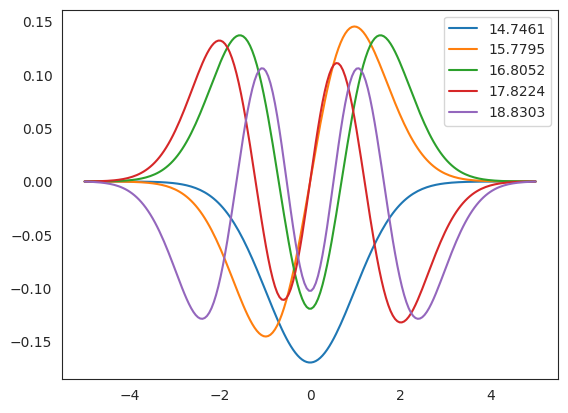
\includegraphics[width=0.8\linewidth]{fig/ks_dft_1d_wfn_ener.png}
    \caption{Wavefunction และพลังงานที่ได้จากการคำนวณ Kohn-Sham DFT สำหรับกรณี 1 มิติ}
    \label{fig:ks_dft_1d_wfn_ener}
\end{figure}

ผู้อ่านที่ต้องการศึกษาโค้ดฉบับสมบูรณ์สามารถดูได้ที่ไฟล์ \inlinehighlight{6_1D_DFT.ipynb} ใน Code Repository ของหนังสือที่
\url{https://github.com/rangsimanketkaew/ml-qm-book-code}

%--------------------------
\section{บันไดของ Jacob สู่สรวงสวรรค์ของความถูกต้องของ DFT}
\label{sec:jacob_ladder}
\idxth{ทฤษฎีฟังก์ชันนอลความหนาแน่น!บันไดของ Jacob}
\idxen{Density Functional Theory!Jacob's ladder}
%--------------------------

\begin{figure}[H]
    \centering
    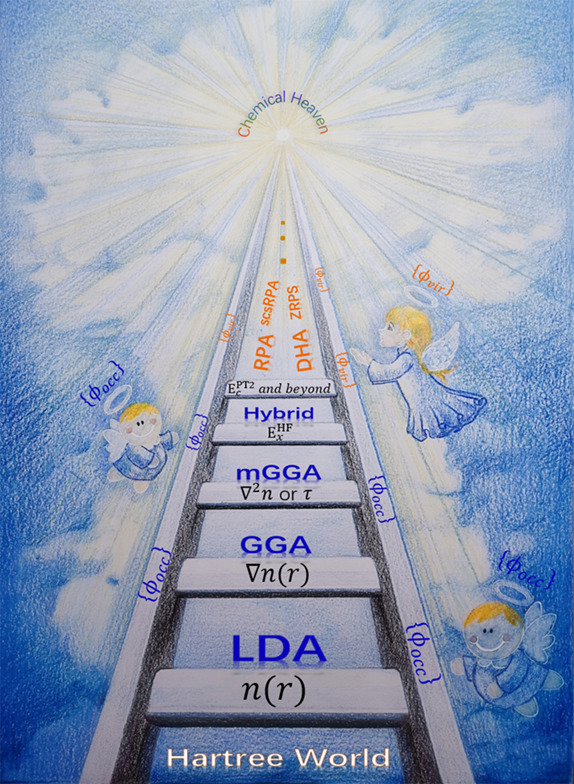
\includegraphics[width=0.75\linewidth]{fig/jacob_ladder.jpg}
    \caption{ขั้นบันไดของ Jacob โดยแต่ละขั้นคือฟังก์ชันนอลของ DFT โดยไล่จากขั้นที่อยู่ด้านล่างสุดคือเทอม Hartree-Fock ซึ่งเป็นองค์ประกอบพื้นฐานของฟังก์ชันนอลทั้งหมดและขั้นสูงสุดคือสวรรค์ทางเคมีซึ่งเปรียบเสมือนเป็นจุดที่แม่นยำที่สุดของวิธี DFT}
    \label{fig:jacob_ladder}
\end{figure}

ในปี 2001 ได้มีบทความงานวิจัยที่นำเสนอไอเดียที่มีการเปรียบเทียบความถูกต้องของวิธี DFT ด้วยบันไดของ Jacob หรือ Jacob's Ladder สำหรับแสดงความถูกต้องและความแม่นยำของการคำนวณโดยไล่ระดับตามขั้นของฟังก์ชันนอล\autocite{perdew2001} ซึ่งฟังก์ชันนอลของ DFT นั้นเป็นการผสมผสานกันของเทอมหลาย ๆ เทอมที่ใช้ในการอธิบายพลังงานต่าง ๆ ภายในโมเลกุล โดยหลัก ๆ ก็จะมีเทอมที่เป็นพลังงานของ Hartree-Fock รวมอยู่ด้วย เมื่อมีการเพิ่มความซับซ้อนให้กับฟังก์ชันนอลโดยรวมเทอมพลังงานอื่น ๆ เข้าไปก็จะเพิ่มความถูกต้องให้กับการคำนวณมากขึ้นเรื่อย ๆ

โดยภาพที่ \ref{fig:jacob_ladder} แสดงขั้นบันไดที่เริ่มจาก Hartree-Fock (HF) ซึ่งบางบทความวิจัยก็เปรียบเทียบว่าเป็นนรก (วิธี HF นั้นให้ความแม่นยำต่ำที่สุดเมื่อเปรียบเทียบกับขั้นบันไดขั้นอื่น ๆ) และขั้นบันไดสุดท้ายคือสววรค์ทางเคมีซึ่งเปรียบเสมือนกับเป็นค่าที่ได้จากการทดลอง (References) จริง ๆ แล้ววิธี HF นั้นแม่นยำในระดับหนึ่งเลยนะครับ โดยผู้เขียนนั้นเคยได้อ่านบทความวิจารณ์ของศาสตราจารย์ Kieron Burke (University of California Irvine) ซึ่งได้สรุปไว้ว่าโดยเฉลี่ยแล้ววิธี HF สามารถทำนายพลังงานรวมของโมเลกุลได้ถูกต้องมากถึง 99\% ส่วนอีก 1\% ที่หายไปนั้นก็คือพลังงานสหสัมพันธ์ (Correlation Energy) อย่างไรก็ตาม วิธี HF นั้นก็มักจะให้ผลการคำนวณการปรับโครงสร้างของโมเลกุลที่ไม่ถูกต้องแม่นยำ เช่น มักจะให้ผลการคำนวณความยาวพันธะหรือการคำนวณความถี่เชิงการสั่นที่คลาดเคลื่อนไปเยอะมาก

เมื่อเวลาผ่านไปก็ได้มีการพัฒนาฟังก์ชันนอลสำหรับ DFT โดยมีการใช้พารามิเตอร์ต่าง ๆ เข้ามาช่วยเพื่อเพิ่มความถูกต้อง เช่น ในยุคแรก ๆ นั้นเริ่มจาก Local Density Approximation (LCD) ซึ่งใช้เพียงแค่ความหนาแน่นของอิเล็กตรอนเพียงอย่างเดียว แล้วในเวลาต่อมาก็ได้มีการใช้ Gradient ของความหนาแน่นของอิเล็กตรอนเข้ามาช่วยจนได้ออกมาเป็นฟังก์ชันนอลแบบ Generalized Gradient Approximation (GGA)\autocite{perdew1996} แล้วตามด้วยการใช้ Hessian ซึ่งได้เป็น Meta GGA (mGGA) แล้วก็มาถึงจุดเปลี่ยนสำคัญคือฟังก์ชันนอลแบบไฮบริด (Hybrid Functional) แล้วก็หลังจากนั้นก็จะเป็นการเพิ่ม Correction เทอมอื่น ๆ โดยใช้วิธีต่าง ๆ เช่น Perturbation หรือ Multireference โดยบันไดขั้นสุดท้ายที่เข้าใกล้ (ต้องใช้คำว่าเข้าใกล้) สวรรค์หรือความถูกต้องมากที่สุดนั้นก็คือฟังก์ชันนอลแบบที่ไม่จำเพาะต่อพื้นที่ (Non-local) นั่นเอง

นอกจากนี้แล้วยังมี Jacob's Ladder ที่เปรียบเทียบวิธีการคำนวณหลาย ๆ วิธีด้วย เช่น เปรียบเทียบระหว่างวิธี DFT กับวิธี Post-HF เช่น เปรียบเทียบกับ Full Configuration Interaction (FCI) ซึ่งเป็นวิธีที่รวมการกระตุ้น (Excitation) ที่มากที่สุดเท่าที่เราต้องการเพื่อทำให้การคำนวณพลังงานสหสัมพันธ์นั้นลู่เข้าได้ง่ายขึ้น

สุดท้ายนี้ผู้เขียนขอให้ความเห็นเพื่อให้ผู้อ่านได้เก็บไว้เป็นแนวคิด 3 ข้อดังนี้
%
\begin{enumerate}[topsep=0pt,noitemsep]\setlength\itemsep{0.5em}
    \item DFT ไม่ใช่วิธีที่ให้ผลการคำนวณที่ถูกต้องและแม่นยำมากที่สุด ยังมีวิธีอื่น ๆ อีกเยอะแยะมากมายที่ให้ผลการคำนวณที่ถูกต้องกว่า ขึ้นอยู่กับโมเลกุลและสิ่งที่เราต้องการคำนวณด้วย

    \item ไม่มีฟังก์ชันนอลไหนที่ดีที่สุดในโลก (ในแง่ของการทำนายคุณสมบัติต่าง ๆ ของโมเลกุล) กล่าวคือบางฟังก์ชันนอลที่แม่นยำในการคำนวณคุณสมบัติหนึ่ง ๆ ของโมเลกุลก็อาจจะไม่แม่นยำในการคำนวณคุณสมบัติอื่น ๆ

    \item การเลือกฟังก์ชันนอลเป็นศิลปะอย่างหนึ่ง ถ้าฟังก์ชันนอลไหนที่ให้ผลที่แม่นยำและใกล้เคียงกับค่าทางการทดลองที่มากที่สุดก็ใช้อันนั้นครับ ดังนั้นจึงเกิดคำถามตามมาว่า \enquote{แล้วเราจะเชื่อถือฟังก์ชันนอลที่เราใช้ได้มากน้อยแค่ไหนถ้าหากสมมติว่าไม่มีผลการทดลองของโมเลกุลนั้น ๆ ให้เราได้เปรียบเทียบ?}
\end{enumerate}
